% Options for packages loaded elsewhere
\PassOptionsToPackage{unicode}{hyperref}
\PassOptionsToPackage{hyphens}{url}
\PassOptionsToPackage{dvipsnames,svgnames,x11names}{xcolor}
%
\documentclass[
]{article}
\usepackage{amsmath,amssymb}
\usepackage{iftex}
\ifPDFTeX
  \usepackage[T1]{fontenc}
  \usepackage[utf8]{inputenc}
  \usepackage{textcomp} % provide euro and other symbols
\else % if luatex or xetex
  \usepackage{unicode-math} % this also loads fontspec
  \defaultfontfeatures{Scale=MatchLowercase}
  \defaultfontfeatures[\rmfamily]{Ligatures=TeX,Scale=1}
\fi
\usepackage{lmodern}
\ifPDFTeX\else
  % xetex/luatex font selection
\fi
% Use upquote if available, for straight quotes in verbatim environments
\IfFileExists{upquote.sty}{\usepackage{upquote}}{}
\IfFileExists{microtype.sty}{% use microtype if available
  \usepackage[]{microtype}
  \UseMicrotypeSet[protrusion]{basicmath} % disable protrusion for tt fonts
}{}
\makeatletter
\@ifundefined{KOMAClassName}{% if non-KOMA class
  \IfFileExists{parskip.sty}{%
    \usepackage{parskip}
  }{% else
    \setlength{\parindent}{0pt}
    \setlength{\parskip}{6pt plus 2pt minus 1pt}}
}{% if KOMA class
  \KOMAoptions{parskip=half}}
\makeatother
\usepackage{xcolor}
\usepackage[margin=2cm]{geometry}
\usepackage{color}
\usepackage{fancyvrb}
\newcommand{\VerbBar}{|}
\newcommand{\VERB}{\Verb[commandchars=\\\{\}]}
\DefineVerbatimEnvironment{Highlighting}{Verbatim}{commandchars=\\\{\}}
% Add ',fontsize=\small' for more characters per line
\usepackage{framed}
\definecolor{shadecolor}{RGB}{251,241,199}
\newenvironment{Shaded}{\begin{snugshade}}{\end{snugshade}}
\newcommand{\AlertTok}[1]{\textcolor[rgb]{0.62,0.00,0.02}{\textbf{#1}}}
\newcommand{\AnnotationTok}[1]{\textcolor[rgb]{0.69,0.38,0.53}{#1}}
\newcommand{\AttributeTok}[1]{\textcolor[rgb]{0.03,0.40,0.47}{#1}}
\newcommand{\BaseNTok}[1]{\textcolor[rgb]{0.71,0.46,0.08}{#1}}
\newcommand{\BuiltInTok}[1]{\textcolor[rgb]{0.56,0.25,0.44}{\textbf{#1}}}
\newcommand{\CharTok}[1]{\textcolor[rgb]{0.60,0.59,0.10}{#1}}
\newcommand{\CommentTok}[1]{\textcolor[rgb]{0.49,0.44,0.39}{#1}}
\newcommand{\CommentVarTok}[1]{\textcolor[rgb]{0.49,0.44,0.39}{#1}}
\newcommand{\ConstantTok}[1]{\textcolor[rgb]{0.80,0.14,0.11}{#1}}
\newcommand{\ControlFlowTok}[1]{\textcolor[rgb]{0.80,0.14,0.11}{\textbf{#1}}}
\newcommand{\DataTypeTok}[1]{\textcolor[rgb]{0.71,0.46,0.08}{#1}}
\newcommand{\DecValTok}[1]{\textcolor[rgb]{0.56,0.25,0.44}{#1}}
\newcommand{\DocumentationTok}[1]{\textcolor[rgb]{0.60,0.59,0.10}{#1}}
\newcommand{\ErrorTok}[1]{\textcolor[rgb]{0.62,0.00,0.02}{\underline{#1}}}
\newcommand{\ExtensionTok}[1]{\textcolor[rgb]{0.27,0.52,0.53}{\textbf{#1}}}
\newcommand{\FloatTok}[1]{\textcolor[rgb]{0.71,0.46,0.08}{#1}}
\newcommand{\FunctionTok}[1]{\textcolor[rgb]{0.69,0.38,0.53}{#1}}
\newcommand{\ImportTok}[1]{\textcolor[rgb]{0.84,0.36,0.05}{#1}}
\newcommand{\InformationTok}[1]{\textcolor[rgb]{0.84,0.36,0.05}{#1}}
\newcommand{\KeywordTok}[1]{\textcolor[rgb]{0.80,0.14,0.11}{\textbf{#1}}}
\newcommand{\NormalTok}[1]{\textcolor[rgb]{0.16,0.16,0.16}{#1}}
\newcommand{\OperatorTok}[1]{\textcolor[rgb]{0.56,0.25,0.44}{#1}}
\newcommand{\OtherTok}[1]{\textcolor[rgb]{0.47,0.45,0.05}{#1}}
\newcommand{\PreprocessorTok}[1]{\textcolor[rgb]{0.03,0.40,0.47}{#1}}
\newcommand{\RegionMarkerTok}[1]{\textcolor[rgb]{0.03,0.40,0.47}{#1}}
\newcommand{\SpecialCharTok}[1]{\textcolor[rgb]{0.47,0.45,0.05}{#1}}
\newcommand{\SpecialStringTok}[1]{\textcolor[rgb]{0.47,0.45,0.05}{#1}}
\newcommand{\StringTok}[1]{\textcolor[rgb]{0.60,0.59,0.10}{#1}}
\newcommand{\VariableTok}[1]{\textcolor[rgb]{0.03,0.40,0.47}{#1}}
\newcommand{\VerbatimStringTok}[1]{\textcolor[rgb]{0.62,0.00,0.02}{#1}}
\newcommand{\WarningTok}[1]{\textcolor[rgb]{0.71,0.46,0.08}{#1}}
\usepackage{longtable,booktabs,array}
\usepackage{calc} % for calculating minipage widths
% Correct order of tables after \paragraph or \subparagraph
\usepackage{etoolbox}
\makeatletter
\patchcmd\longtable{\par}{\if@noskipsec\mbox{}\fi\par}{}{}
\makeatother
% Allow footnotes in longtable head/foot
\IfFileExists{footnotehyper.sty}{\usepackage{footnotehyper}}{\usepackage{footnote}}
\makesavenoteenv{longtable}
\setlength{\emergencystretch}{3em} % prevent overfull lines
\providecommand{\tightlist}{%
  \setlength{\itemsep}{0pt}\setlength{\parskip}{0pt}}
\setcounter{secnumdepth}{-\maxdimen} % remove section numbering
% definitions for citeproc citations
\NewDocumentCommand\citeproctext{}{}
\NewDocumentCommand\citeproc{mm}{%
  \begingroup\def\citeproctext{#2}\cite{#1}\endgroup}
\makeatletter
 % allow citations to break across lines
 \let\@cite@ofmt\@firstofone
 % avoid brackets around text for \cite:
 \def\@biblabel#1{}
 \def\@cite#1#2{{#1\if@tempswa , #2\fi}}
\makeatother
\newlength{\cslhangindent}
\setlength{\cslhangindent}{1.5em}
\newlength{\csllabelwidth}
\setlength{\csllabelwidth}{3em}
\newenvironment{CSLReferences}[2] % #1 hanging-indent, #2 entry-spacing
 {\begin{list}{}{%
  \setlength{\itemindent}{0pt}
  \setlength{\leftmargin}{0pt}
  \setlength{\parsep}{0pt}
  % turn on hanging indent if param 1 is 1
  \ifodd #1
   \setlength{\leftmargin}{\cslhangindent}
   \setlength{\itemindent}{-1\cslhangindent}
  \fi
  % set entry spacing
  \setlength{\itemsep}{#2\baselineskip}}}
 {\end{list}}
\usepackage{calc}
\newcommand{\CSLBlock}[1]{\hfill\break\parbox[t]{\linewidth}{\strut\ignorespaces#1\strut}}
\newcommand{\CSLLeftMargin}[1]{\parbox[t]{\csllabelwidth}{\strut#1\strut}}
\newcommand{\CSLRightInline}[1]{\parbox[t]{\linewidth - \csllabelwidth}{\strut#1\strut}}
\newcommand{\CSLIndent}[1]{\hspace{\cslhangindent}#1}
\usepackage{xcolor}
\definecolor{GbGreenNt}{HTML}{98971a}
\definecolor{GbBlueNt}{HTML}{458588}
\definecolor{GbGrayNt}{HTML}{928374}
\definecolor{GbBlueDk}{HTML}{076678}
\definecolor{GbGrey}{HTML}{504945}
\definecolor{GbFg4}{HTML}{7c6f64}
\definecolor{GbFg3}{HTML}{665c54}
\definecolor{GbFg2}{HTML}{504945}
\definecolor{GbFg1}{HTML}{3c3836}
\usepackage{mathtools}

\usepackage{subcaption} 
\usepackage{tikz}
\usetikzlibrary{shapes.geometric, arrows, positioning}

\tikzstyle{process} = [rectangle, minimum width=2cm, minimum height=1cm, text centered, draw=black]
\tikzstyle{data} = [trapezium, trapezium left angle=70, trapezium right angle=110, minimum width=1.5cm, minimum height=1cm, text centered, draw=black]
\tikzstyle{arrow} = [->, >=latex]
\tikzstyle{thick-arrow} = [thick, ->, >=latex]
\tikzstyle{dashed-arrow} = [dashed, ->]
\tikzstyle{node} = [rectangle, draw=black, minimum width=1cm, minimum height=1cm, text centered]

\tikzstyle{box} = [rectangle, draw, rounded corners, text centered, minimum height=1cm]

\usepackage{pgfplots}
\pgfplotsset{compat=1.18}
\usepackage{pgfplotstable}

\usepackage{hyperref}
\hypersetup{
    colorlinks=true, %set true if you want colored links
    linktoc=all,     %set to all if you want both sections and subsections linked
    linkcolor=GbBlueNt,    % Internal links (e.g., section links)
    citecolor=GbGreenNt,   % Citation links
    urlcolor=GbBlueDk      % External URL links
}

\usepackage{caption}
\usepackage{algorithm}
\usepackage{algpseudocode}

\newcommand{\Desc}[2]{\hspace*{\algorithmicindent} \makebox[14.5em][l]{#1}\parbox[t]{32em}{#2}}

\usepackage[style=iso]{datetime2}

% Float figures
\usepackage{float}
\let\origfigure\figure
\let\endorigfigure\endfigure
\renewenvironment{figure}[1][2] {
    \expandafter\origfigure\expandafter[H]
} {
    \endorigfigure
}

\newcommand*\Bb{\mathbb{B}}
\newcommand*\Zb{\mathbb{Z}}
\newcommand*\Fb{\mathbb{F}}
\newcommand*\Nb{\mathbb{N}}
\newcommand*\Rb{\mathbb{R}}
\newcommand*\Eb{\mathbb{E}}
\newcommand*\Gb{\mathbb{G}}
\newcommand*\Ac{\mathcal{A}}
\newcommand*\Bc{\mathcal{B}}
\newcommand*\Cc{\mathcal{C}}
\newcommand*\Dc{\mathcal{D}}
\newcommand*\Ec{\mathcal{E}}
\newcommand*\Rc{\mathcal{R}}
\newcommand*\Oc{\mathcal{O}}
\newcommand*\Uc{\mathcal{U}}
\newcommand*\Mc{\mathcal{M}}
\newcommand*\Pc{\mathcal{P}}
\newcommand*\Vc{\mathcal{V}}
\newcommand*\Sc{\mathcal{S}}
\newcommand*\Hc{\mathcal{H}}

\renewcommand*\a{\alpha}
\renewcommand*\b{\beta}
\renewcommand*\d{\delta}
\newcommand*\e{\epsilon}
\renewcommand*\l{\lambda}
\newcommand*\p{\phi}
\renewcommand*\o{\omega}
\newcommand*\ps{\psi}
\renewcommand*\S{\Sigma}

\renewcommand*\mod{\bmod}
\newcommand*\cat{\mathbin{+\mkern-10mu+}}
\newcommand*\bor{\mathbin{\&\mkern-7mu\&}}
\newcommand*\xor{\oplus}
\newcommand*\meq{\stackrel{?}{=}}
\newcommand*\iso{\cong}
\newcommand{\qed}{\hfill \ensuremath{\Box}}
\newcommand{\defend}{\hfill \ensuremath{\triangle}}
\newcommand*{\then}{\implies}

\newcommand*\algind{\hspace*{\algorithmicindent}}
\newcommand*\algindd{\algind \algind}

\newcommand{\textblue}[1]{\textcolor{GbBlueDk}{#1}}
\newcommand{\mathblue}[1]{\mathcolor{GbBlueDk}{#1}}
\newcommand{\textgrey}[1]{\textcolor{GbGrey}{#1}}
\newcommand{\mathgrey}[1]{\mathcolor{GbGrey}{#1}}
\newcommand{\floor}[1]{\left \lfloor #1 \right \rfloor }
\newcommand{\ceil}[1]{\left \lceil #1 \right \rceil }
\renewcommand{\vec}[1]{ \boldsymbol{#1} }
\newcommand{\ran}[1]{ \mathrm{#1} }
\newcommand{\ranvec}[1]{ \boldsymbol{\ran{#1}} }
\newcommand{\dotp}[2]{ \langle #1, #2 \rangle }
\newcommand{\ip}[2]{ \langle #1, #2 \rangle }
\newcommand{\IK}[2]{ \mathrm{I.K} }

\newcommand*{\negl}{\text{negl}}
\newcommand*{\poly}{\text{poly}}
\newcommand*{\from}{\gets}
\newcommand*{\pp}{\mathrm{pp}}
\newcommand*{\acc}{\mathrm{acc}}
\newcommand*{\ToInstance}{\mathrm{\text{T\scriptsize O}\text{I\scriptsize NSTANCE}}}
\newcommand*{\Prover}{\mathrm{\text{P\scriptsize ROVER}}}
\newcommand*{\Verifier}{\mathrm{\text{V\scriptsize ERIFIER}}}
\newcommand*{\Setup}{\mathrm{\text{S{\scriptsize ETUP}}}}
\newcommand*{\Generator}{\mathrm{\text{G{\scriptsize ENERATOR}}}}
\newcommand*{\Trim}{\mathrm{\text{T{\scriptsize RIM}}}}
\newcommand*{\Commit}{\mathrm{\text{C{\scriptsize OMMIT}}}}
\newcommand*{\Decider}{\mathrm{\text{D{\scriptsize ECIDER}}}}
\newcommand*{\SNARKProver}{\mathrm{\text{SNARK}}.\Prover}
\newcommand*{\SNARKVerifier}{\mathrm{\text{SNARK}}.\Verifier}
\newcommand*{\SNARKVerifierSlow}{\mathrm{\text{SNARK}}.\mathrm{\text{V\scriptsize ERIFIER}\text{S\scriptsize LOW}}}
\newcommand*{\SNARKVerifierFast}{\mathrm{\text{SNARK}}.\mathrm{\text{V\scriptsize ERIFIER}\text{F\scriptsize AST}}}
\newcommand*{\IVCProver}{\mathrm{\text{IVC}}.\Prover}
\newcommand*{\IVCVerifier}{\mathrm{\text{IVC}}.\Verifier}
\newcommand*{\AS}{\text{AS}}
\newcommand*{\ASGenerator}{\AS.\Generator}
\newcommand*{\ASSetup}{\AS.\Setup}
\newcommand*{\ASProver}{\AS.\Prover}
\newcommand*{\ASVerifier}{\AS.\Verifier}
\newcommand*{\ASDecider}{\AS.\Decider}
\newcommand*{\PC}{\text{PC}}
\newcommand*{\PCSetup}{\PC.\Setup}
\newcommand*{\PCTrim}{\PC.\Trim}
\newcommand*{\PCCommit}{\PC.\Commit}
\newcommand*{\PCOpen}{\PC.\mathrm{\text{O\scriptsize PEN}}}
\newcommand*{\PCCheck}{\PC.\mathrm{\text{C\scriptsize HECK}}}
\newcommand*{\PCDL}{\text{PC}_{\text{DL}}}
\newcommand*{\PCDLSetup}{\PCDL.\Setup}
\newcommand*{\PCDLTrim}{\PCDL.\Trim}
\newcommand*{\PCDLCommit}{\PCDL.\Commit}
\newcommand*{\PCDLOpen}{\PCDL.\mathrm{\text{O\scriptsize PEN}}}
\newcommand*{\PCDLSuccinctCheck}{\PCDL.\mathrm{\text{S{\scriptsize UCCINCT}C{\scriptsize HECK}}}}
\newcommand*{\PCDLCheck}{\PCDL.\mathrm{\text{C\scriptsize HECK}}}
\newcommand*{\ASDL}{\text{AS}_{\text{DL}}}
\newcommand*{\ASDLSetup}{\ASDL.\Setup}
\newcommand*{\ASDLIndexer}{\ASDL.\mathrm{\text{I\scriptsize NDEXER}}}
\newcommand*{\ASDLCommonSubroutine}{\ASDL.\mathrm{\text{C{\scriptsize OMMON}S{\scriptsize UBROUTINE}}}}
\newcommand*{\ASDLProver}{\ASDL.\mathrm{\text{P\scriptsize ROVER}}}
\newcommand*{\ASDLVerifier}{\ASDL.\mathrm{\text{V\scriptsize ERIFIER}}}
\newcommand*{\ASDLDecider}{\ASDL.\mathrm{\text{D\scriptsize ECIDER}}}
\newcommand*{\CM}{\mathrm{\text{CM}}}
\newcommand*{\CMSetup}{\CM.\Setup}
\newcommand*{\CMTrim}{\CM.\Trim}
\newcommand*{\CMCommit}{\CM.\Commit}

\newcommand*\Result{\mathbf{Result}}
\newcommand*\Option{\mathbf{Option}}
\newcommand*\Acc{\mathbf{Acc}}
\newcommand*\Instance{\mathbf{Instance}}
\newcommand*\Proof{\mathbf{Proof}}
\newcommand*\Witness{\mathbf{Witness}}
\newcommand*\PublicInfo{\mathbf{PublicInputs}}
\newcommand*\PublicInputs{\mathbf{PublicInputs}}
\newcommand*\Circuit{\mathbf{Circuit}}
\newcommand*\AccHiding{\mathbf{AccHiding}}
\newcommand*\EvalProof{\mathbf{EvalProof}}


\ifLuaTeX
  \usepackage{selnolig}  % disable illegal ligatures
\fi
\usepackage{bookmark}
\IfFileExists{xurl.sty}{\usepackage{xurl}}{} % add URL line breaks if available
\urlstyle{same}
\hypersetup{
  pdftitle={Investigating IVC with Accumulation Schemes},
  pdfauthor={Rasmus Kirk Jakobsen - 201907084},
  colorlinks=true,
  linkcolor={black},
  filecolor={Maroon},
  citecolor={black},
  urlcolor={GbBlueDk},
  pdfcreator={LaTeX via pandoc}}

\title{Investigating IVC with Accumulation Schemes\thanks{I would like
to express my gratitude to Jesper Buus Nielsen and Hamidreza
Khoshakhlagh for their invaluable help in answering many of my
questions.}}
\author{Rasmus Kirk Jakobsen - 201907084}
\date{2025-01-29 - 17:47:42 UTC}

\begin{document}
\maketitle

{
\hypersetup{linkcolor=black}
\setcounter{tocdepth}{3}
\tableofcontents
}
\section{Introduction}\label{introduction}

Incrementally Verifiable Computation (IVC) has seen increased practical
usage, notably by the Mina{[}\citeproc{ref-mina}{2025}{]} blockchain to
achieve a succinct blockchain. This is enabled by increasingly efficient
recursive proof systems, one of the most used in practice is based on
{[}\citeproc{ref-halo}{Bowe et al. 2019}{]}, which includes Halo2 by the
Electric Coin Company (to be used in Zcash) and Kimchi developed and
used by Mina. Both can be broken down into the following main
components:

\begin{itemize}
\tightlist
\item
  \textbf{Plonk}: A general-purpose, potentially zero-knowledge, SNARK.
\item
  \textbf{\(\PCDL\)}: A Polynomial Commitment Scheme in the Discrete Log
  setting.
\item
  \textbf{\(\ASDL\)}: An Accumulation Scheme in the Discrete Log
  setting.
\item
  \textbf{Pasta}: A cycle of elliptic curves, Pallas and Vesta,
  collectively known as Pasta.
\end{itemize}

This project is focused on the components of \(\PCDL\) and \(\ASDL\)
from the 2020 paper \emph{``Proof-Carrying Data from Accumulation
Schemes''}{[}\citeproc{ref-pcd}{Bünz et al. 2020}{]}. The project
explores the theoretical aspects of the scheme described in the paper
document with a corresponding Rust implementation. Both the report and
the implementation can be found in the project's
repository{[}\citeproc{ref-repo}{Jakobsen 2025}{]}.

\subsection{Prerequisites}\label{prerequisites}

Basic knowledge of elliptic curves, groups, interactive arguments is
assumed, along with familiarity with SNARKs, in the following text. The
polynomial commitment scheme heavily relies on the Inner Product Proof
from the Bulletproofs protocol. If needed, refer to the following
resources:

\begin{itemize}
\tightlist
\item
  Section 3 in the original
  Bulletproofs{[}\citeproc{ref-bulletproofs}{Bünz et al. 2017}{]} paper
\item
  From Zero (Knowledge) to Bulletproofs
  writeup{[}\citeproc{ref-from0k2bp}{Gibson 2022}{]}
\item
  Rust Dalek Bulletproofs implementation
  notes{[}\citeproc{ref-dalek-docs}{Valence et al. 2023}{]}
\item
  Section 4.1 of my bachelors
  thesis{[}\citeproc{ref-hacspec-bulletproofs}{Jakobsen and Larsen
  2022}{]}
\end{itemize}

\subsection{Background and Motivation}\label{background-and-motivation}

The following subsections introduce the concept of Incrementally
Verifiable Computation (IVC) along with some background concepts. These
concepts lead to the introduction of accumulation schemes and polynomial
commitment schemes, the main focus of this paper. Accumulation schemes,
in particular, will be demonstrated as a means to create more flexible
IVC constructions compared to previous approaches, allowing IVC that
does not depend on a trusted setup.

As such, these subsections aim to provide an overview of the evolving
field of IVC, the succinct proof systems that lead to its construction,
and the role of accumulation schemes as an important cryptographic
primitive with practical applications.

\subsubsection{Proof Systems}\label{proof-systems}

An Interactive Proof System consists of two Interactive Turing Machines:
a computationally unbounded Prover, \(\Pc\), and a polynomial-time
bounded Verifier, \(\Vc\). The Prover tries to convince the Verifier of
a statement \(x \in L\), with language \(L\) in NP. The following
properties must be true:

\begin{itemize}
\item
  \textbf{Completeness:}
  \(\forall \Pc \in ITM, x\in L \implies \Pr[\Vc_{out} = \bot] \leq \epsilon(x)\)

  For all honest provers, \(\Pc\), where \(x\) is true, the probability
  that the verifier remains unconvinced is negligible in the length of
  \(x\).
\item
  \textbf{Soundness:}
  \(\forall \Pc^* \in ITM, x \notin L \implies \Pr[\Vc_{out} = \top] \leq \epsilon(x)\)

  For all provers, honest or otherwise, \(\Pc^*\), that try to convince
  the verifier of a claim, \(x\), that is not true, the probability that
  the verifier will be convinced is negligible in the length of \(x\).
\end{itemize}

An Interactive Argument is very similar, but the honest and malicious
prover are now polynomially bounded and receives a witness, \(w\):

\begin{itemize}
\tightlist
\item
  \textbf{Completeness}:
  \(\forall \Pc(w) \in PPT, x\in L \implies \Pr[\Vc_{out} = \bot] \leq \epsilon(x)\)
\item
  \textbf{Soundness}:
  \(\forall \Pc^* \in PPT, x \notin L \implies \Pr[\Vc_{out} = \top] \leq \epsilon(x)\)
\end{itemize}

Proofs of knowledge are another type of Proof System, here the prover
claims to know a specific \emph{witness}, \(w\), for a statement \(x\).
Let \(x \in
L\) and \(W(x)\) be the set of witnesses for \(x\) that should be
accepted in the proof. This allows us to define the following relation:
\(R = \{ (x,w)
: x \in L , w \in W(x) \}\)

A proof of knowledge for relation \(R\) with is a two party protocol
\((P, \Vc)\) with the following two properties:

\begin{itemize}
\tightlist
\item
  \textbf{Knowledge Completeness:}
  \(\Pr[\Pc(w) \iff \Vc_{out} = 1] = 1\), i.e.~as in Interactive Proof
  Systems, after an interaction between the prover and verifier the
  verifier should be convinced with certainty.\\
\item
  \textbf{Knowledge Soundness:} Loosely speaking, Knowledge Soundness
  requires the existence of an efficient extractor \(\Ec\) that, when
  given a possibly malicious prover \(\Pc^*\) as input, can extract a
  valid witness with probability at least as high as the probability
  that \(\Pc^\) convinces the verifier \(\Vc\).
\end{itemize}

The above proof systems may be \emph{zero-knowledge}, which in loose
terms means that anyone looking at the transcript, that is the
interaction between prover and verifier, will not be able to tell the
difference between a real transcript and one that is simulated. This
ensures that an adversary gains no new information beyond what they
could have computed on their own. We now define the property more
formally:

\begin{itemize}
\tightlist
\item
  \textbf{Zero-knowledge:}
  \(\forall \Vc^*(\delta). \exists S_{\Vc^*}(x) \in PPT. S_{\Vc^*} \sim^C (\Pc,\Vc^*)\)
\end{itemize}

\(\Vc^*\) denotes a prover, honest or otherwise, \(\d\) represents
information that \(\Vc^*\) may have from previous executions of the
protocol and \((\Pc,\Vc^*)\) denotes the transcript between the honest
prover and (possibly) malicious verifier. There are three kinds of
zero-knowledge:

\begin{itemize}
\tightlist
\item
  \textbf{Perfect Zero-knowledge:}
  \(\forall \Vc^*(\delta). \exists S_{\Vc^*}(x) \in PPT. S_{\Vc^*} \sim^\Pc (\Pc,\Vc^*)\),
  the transcripts \(S_{\Vc^*}(x)\) and \((\Pc,\Vc^*)\) are perfectly
  indistinguishable.
\item
  \textbf{Statistical Zero-knowledge:}
  \(\forall \Vc^*(\delta). \exists S_{\Vc^*}(x) \in PPT. S_{\Vc^*} \sim^S (\Pc,\Vc^*)\),
  the transcripts \(S_{\Vc^*}(x)\) and \((\Pc,\Vc^*)\) are statistically
  indistinguishable.
\item
  \textbf{Computational Zero-knowledge:}
  \(\forall \Vc^*(\delta). \exists S_{\Vc^*}(x) \in PPT. S_{\Vc^*} \sim^C (\Pc,\Vc^*)\),
  the transcripts \(S_{\Vc^*}(x)\) and \((\Pc,\Vc^*)\) are
  computationally indistinguishable, i.e.~no polynomially bounded
  adversary \(\Ac\) can distinguish them.
\end{itemize}

\paragraph{Fiat-Shamir Heuristic}\label{fiat-shamir-heuristic}

The standard Fiat-Shamir heuristic is used to turn interactive protocols
non-interactive. The Fiat-Shamir heuristic turns a public-coin
interactive proof into a non-interactive proof, by replacing all
uniformly random values sent from the verifier to the prover with calls
to a non-interactive random oracle. In practice, a cryptographic hash
function, \(\rho\), is used. Composing proof systems will sometimes
require \emph{domain-separation}, whereby random oracles used by one
proof system cannot be accessed by another proof system. This is the
case for the zero-finding game that will be used in the soundness
discussions of implemented accumulation scheme \(\ASDL\). In practice
one can have a domain specifier, for example \(0, 1\), prepended to each
message that is hashed using \(\rho\):
\[ \rho_0(m) &= \rho(0 \cat m) \quad \rho_1(m) &= \rho(1 \cat m)\]

\paragraph{SNARKS}\label{snarks}

SNARKs - \textbf{S}uccinct \textbf{N}on-interactive \textbf{AR}guments
of \textbf{K}nowledge - have seen increased usage due to their
application in blockchains and cryptocurrencies. They usually also
function as so-called general-purpose proof schemes. This means that,
given any solution to an NP-problem, it will produce a proof that the
prover knows the solution to said NP-problem. Most SNARKs also allow for
zero-knowledge arguments, making them zk-SNARKs.

More concretely, imagine that Alice has todays sudoku problem \(x\): She
claims to have a solution to this problem, her witness, \(w\), and want
to convince Bob without having to send all of it. She could then use a
SNARK to create a proof to convince Bob. To do this she must first
encode the sudoku verifier as a circuit \(R_x\), which includes public
inputs, such as today's sudoku values/positions, etc, and then give the
SNARK prover (\(\SNARKProver\)) \(R_x(w,w')\). Finally she can send this
proof, \(\pi\), to Bob along with the public sudoku verifying circuit,
\(R_x\), and he can check the proof and be convinced using the snark
verifier (\(\SNARKVerifier\)).

Importantly, the succinct part of the name means that the proof size and
verification time must be sub-linear. This allows SNARKs to be directly
used for \emph{Incrementally Verifiable Computation}.

\paragraph{Trusted and Untrusted
Setups}\label{trusted-and-untrusted-setups}

Many SNARK constructions, such as the original Plonk specification,
depend on a Trusted Setup to ensure soundness. For Plonk, this arises
from the KZG{[}\citeproc{ref-kzg}{Kate et al. 2010}{]} commitments used.
These commitments lets the SNARK verifier enjoy sub-linear verification
time, but at the cost of requiring a trusted setup while \(\PCDL\) only
relies on an untrusted setup. A trusted setup creates a
\textbf{Structured Reference String} (SRS) with a specific internal
structure.

An untrusted setup, however, creates a \textbf{Uniform Random String} of
the form: \[\text{URS} = \{ \a_1G, \a_2G, \dots, \a_DG \}\] Where \(D\)
represents the maximum degree bound of a polynomial and \(G\) is a
generator. The URS must consist of only generators and all the
\(\vec{\a}\) scalars must be uniformly random. \(\PCDL\) is then sound,
provided that no adversary knows the \(\vec{\a}\) scalars. Extracting
\(\vec{\a}\) from the URS would require solving the Discrete Logarithm
problem, which is assumed to be hard.

To generate the URS transparently, a collision-resistant hash function
\(\Hc : \Bb^* \to \Eb(\Fb_q)\) can be used to produce the generators.
The URS can then be derived using a genesis string \(s\):
\[\text{URS} = \{ \Hc(s \cat 1), \Hc(s \cat 2), \dots, \Hc(s \cat D) \}\]
This is the method used in the implementation, as mentioned in the
implementation section further down.

\paragraph{Bulletproofs}\label{bulletproofs}

In 2017, the Bulletproofs paper{[}\citeproc{ref-bulletproofs}{Bünz et
al. 2017}{]} was released. Bulletproofs relies on the hardness of the
Discrete Logarithm problem, and allows for an untrusted setup to
generate the Common Reference String. It has logarithmic proof size, and
lends itself well efficient range proofs. It's also possible to generate
proofs for arbitrary circuits, but with less efficiency.

At the heart of Bulletproofs lies the Inner Product Argument (IPA),
wherein a prover proves he knows two vectors,
\(\vec{a}, \vec{b} \in \Fb_q^n\), with commitment \(C \in \Eb(\Fb_q)\),
and their corresponding inner product, \(c = \ip{\vec{a}}{\vec{b}}\). It
creates this non-interactive proof, with only \(\lg(n)\) size, by
compressing the point and vectors \(\lg(n)\) times. Unfortunately, the
IPA, and by extension Bulletproofs, suffer from linear verification
time, making them unsuitable for IVC.

\subsubsection{Incrementally Verifiable
Computation}\label{incrementally-verifiable-computation}

Valiant originally described IVC in his 2008
paper{[}\citeproc{ref-valiant}{Valiant 2008}{]} in the following way:

\begin{quote}
\color{GbGrey}

\textit{Suppose humanity needs to conduct a very long computation which will span
superpolynomially many generations. Each generation runs the computation
until their deaths when they pass on the computational configuration to the
next generation. This computation is so important that they also pass on a
proof that the current configuration is correct, for fear that the following
generations, without such a guarantee, might abandon the project. Can this
be done?}

\end{quote}

That is, if we run a computation for 100's of years only for it to
output 42, is there a way for us to know that the output of said
computation is correct, without taking the time to redo all that
computation? In order to do this, the verification of the final output
of the computation must be much smaller than simply running the
computation again. Valiant creates the concepts of IVC and argues that
IVC can be used to achieve the above goal.

Recently the concept of IVC has seen renewed interest with
cryptocurrencies, as this concept lends itself well to the structure of
blockchains. This allows a blockchain node to omit all previous
transaction history in favour of only a single state, for example,
containing all current account balances. This is commonly called a
\emph{succinct blockchain}, one such blockchain is
Mina{[}\citeproc{ref-mina}{2025}{]}.

In order to achieve IVC, you need a function \(F(x) \in S \to S\) along
with some initial state \(s_0 \in S\). Then you can call \(F(x)\) to
generate a series of \(s\)'s, \(\vec{s} \in S^{n+1}\):

\begin{figure}[!H]
\centering
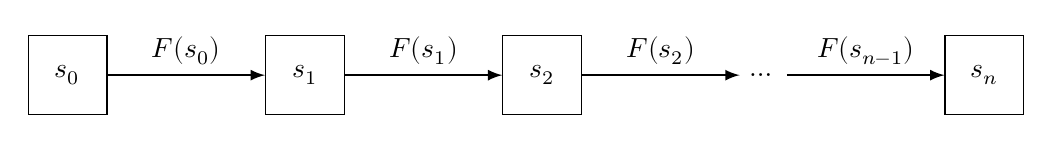
\begin{tikzpicture}[node distance=2cm]

  % Nodes
  \node (s0) [node] {$s_0$};
  \node (s1) [node, right=of s0] {$s_1$};
  \node (s2) [node, right=of s1] {$s_2$};
  \node (dots) [right=2cm of s2] {$\dots$};
  \node (sn) [node, right=2cm of dots] {$s_n$};

  % Arrows with labels
  \draw[thick-arrow] (s0) -- node[above] {$F(s_0)$} (s1);
  \draw[thick-arrow] (s1) -- node[above] {$F(s_1)$} (s2);
  \draw[thick-arrow] (s2) -- node[above] {$F(s_2)$} (dots);
  \draw[thick-arrow] (dots) -- node[above] {$F(s_{n-1})$} (sn);

\end{tikzpicture}
\caption{
  A visualization of the relationship between $F(x)$ and $\vec{s}$ in a non-IVC setting.
}
\end{figure}

In a blockchain setting, you might imagine any \(s_i \in \vec{s}\) as a
set of accounts with corresponding balances, and the transition
function\footnote{In the blockchain setting, the transition function
  would also take an additional input representing new transactions,
  \(F(x: S, T: \Pc(T))\).} \(F(x)\) as the computation happening when a
new block is created and therefore a new state, or set of accounts,
\(s_i\) is computed.

In the IVC setting, we have a proof, \(\pi\), associated with each
state, so that anyone can take only a single pair \((s_m, \pi_m)\) along
with the initial state and transition function (\(s_0, F(x)\)) and
verify that said state was computed correctly.

\begin{figure}[!H]
\centering
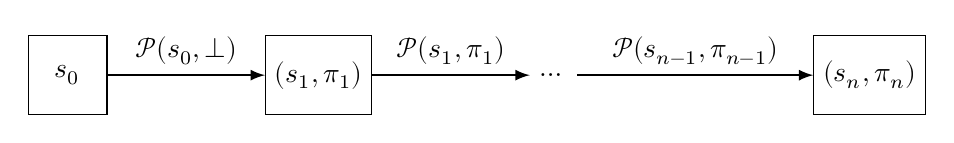
\begin{tikzpicture}[node distance=2cm]

  % Nodes
  \node (s0) [node] {$s_0$};
  \node (s1) [node, right=of s0] {$(s_1, \pi_1)$};
  \node (dots) [right=2cm of s1] {$\dots$};
  \node (sn) [node, right=3cm of dots] {$(s_n, \pi_n)$};

  % Arrows with labels
  \draw[thick-arrow] (s0) -- node[above] {$\Pc(s_0, \bot)$} (s1);
  \draw[thick-arrow] (s1) -- node[above] {$\Pc(s_1, \pi_1)$} (dots);
  \draw[thick-arrow] (dots) -- node[above] {$\Pc(s_{n-1}, \pi_{n-1})$} (sn);

\end{tikzpicture}
\caption{
  A visualization of the relationship between $F, \vec{s}$ and $\vec{\pi}$
  in an IVC setting using traditional SNARKs. $\Pc(s_i, \pi_i)$ denotes
  $\SNARKProver(R_F, s_{i-1}, \pi_{i-1}) = (s_i, \pi_i)$ where $R_F$ is the
  transition function $F$ expressed as a circuit.
}
\end{figure}

The proof \(\pi_i\) describes the following claim:

\begin{quote}
\color{GbGrey}

\textit{"The current state $s_i$ is computed from applying the function,
$F$, $i$ times to $s_0$ ($s_i = F^i(s_0) = F(s_{i-1})$) and the associated
proof $\pi_{i-1}$ for the previous state is valid."}

\end{quote}

Or more formally, \(\pi_i\) is a proof of the following claim, expressed
as a circuit \(R\):
\[R := \text{I.K.} \; \pi_{n-1} \; \text{ s.t. } \; s_i \meq F(s_{i-1}) \; \land \; (s_{i-1} \meq s_0 \lor \SNARKVerifier(R_F, s_{i-1}, \pi_{i-1}) \meq \top))\]
Note that \(R_F, s_{i-1}, s_0\) are not quantified above, but are public
values. The \(\SNARKVerifier\) represents the verification circuit in
the proof system we're using. This means, that we're taking the
verifier, representing it as a circuit, and then feeding it to the
prover. This is not a trivial task in practice! Note also, that the
verification time must be sub-linear to achieve an IVC scheme, otherwise
the verifier could just have computed \(F^{n+1}(s_0)\) themselves, as
\(s_0\) and \(F(x)\) necessarily must be public.

To see that the above construction works, observe that \(\pi_1, \dots,
\pi_n\) proves: \[
\begin{alignedat}{7}
  &\text{I.K.} \; \pi_{n-1} \; &&\text{ s.t. } \; &&s_n     &&= F(s_{n-1}) \; &&\land \; (s_{n-1} = s_0  &&\lor \SNARKVerifier(R, s_{n-1}, \pi_{n-1}) = \top), \\
  &\text{I.K.} \; \pi_{n-2} \; &&\text{ s.t. } \; &&s_{n-1} &&= F(s_{n-2}) \; &&\land \; (s_{n-2} = s_0  &&\lor \SNARKVerifier(R, s_{n-2}, \pi_{n-2}) = \top), \; \dots \\
  &                            &&              \; &&s_1     &&= F(s_0)     \; &&\land \; (s_0 = s_0      &&\lor \SNARKVerifier(R, s_0, \pi_0) = \top)
\end{alignedat}
\] Which means that: \[
\begin{alignedat}{4}
  &\SNARKVerifier(R, s_n, \pi_n) = \top \implies \\
  &s_n = F(s_{n-1}) \; \land \; \\
  &\SNARKVerifier(R, s_{n-1}, \pi_{n-1}) = \top \; \land \; \\
  &s_{n-1} = F(s_{n-2}) \implies \dots \\
  &\SNARKVerifier(R, s_1 \pi_1) = \top \implies \\
  &s_1 = F(s_0)
\end{alignedat}
\] Thus, by induction \(s_n = F^n(s_0)\)

\subsubsection{Polynomial Commitment
Schemes}\label{polynomial-commitment-schemes}

In the section SNARKs section, general-purpose proof schemes were
described. Modern general-purpose (zero-knowledge) proof schemes, such
as Sonic{[}\citeproc{ref-sonic}{Maller et al. 2019}{]},
Plonk{[}\citeproc{ref-plonk}{Gabizon et al. 2019}{]} and
Marlin{[}\citeproc{ref-marlin}{Chiesa et al. 2019}{]}, commonly use
\emph{Polynomial Commitment Schemes} (PCSs) for creating their proofs.
This means that different PCSs can be used to get security under weaker
or stronger assumptions.

\begin{itemize}
\tightlist
\item
  \textbf{KZG PCSs:} Uses a trusted setup, this would give you a
  traditional SNARK.
\item
  \textbf{Bulletproofs PCSs:} Uses an untrusted setup, assumes secure if
  the Discrete Log problem is hard, the verifier is linear.
\item
  \textbf{FRI PCSs:} Also uses an untrusted setup, assumes secure one
  way functions exist. It has a higher overhead than PCSs based on the
  Discrete Log assumption, but since it's not based on the Discrete Log
  assumption, and instead assumes that secure one-way functions exist,
  you end up with a quantum secure PCS.
\end{itemize}

A PCS allows a prover to prove to a verifier that a committed polynomial
evaluates to a certain value, \(v\), given an evaluation input
\(z\).There are four main functions used to prove this (\(\PCTrim\)
omitted as it's unnecessary):

\begin{itemize}
\item
  \(\PCSetup(\l, D)^\rho \to \pp\)

  The setup routine. Given security parameter \(\l\) in unary and a
  maximum degree bound \(D\). Creates the public parameters \(\pp_\PC\).
\item
  \(\PCCommit(p: \Fb^{d'}_q[X], d: \Nb, \o: \Option(\Fb_q)) \to \Eb(\Fb_q)\)

  Commits to a degree-\(d'\) polynomial \(p\) with degree bound \(d\)
  where \(d'
  \leq d\) using optional hiding \(\o\).
\item
  \(\PCOpen^\rho(p: \Fb^{d'}_q[X], C: \Eb(\Fb_q), d: \Nb, z: \Fb_q, \o: \Option(\Fb_q)) \to \EvalProof\)

  Creates a proof, \(\pi \in \EvalProof\), that the degree \(d'\)
  polynomial \(p\), with commitment \(C\), and degree bound \(d\) where
  \(d' \leq d\), evaluated at \(z\) gives \(v = p(z)\), using the hiding
  input \(\o\) if provided.
\item
  \(\PCCheck^\rho(C: \Eb(\Fb_q), d: \Nb, z: \Fb_q, v: \Fb_q, \pi: \EvalProof) \to \Result(\top, \bot)\)

  Checks the proof \(\pi\) that claims that the degree \(d'\) polynomial
  \(p\), with commitment \(C\), and degree bound \(d\) where
  \(d' \leq d\), evaluates to \(v = p(z)\).
\end{itemize}

Any NP-problem, \(X \in NP\), with a witness \(w\) can be compiled into
a circuit \(R_X\). This circuit can then be fed to a general-purpose
proof scheme prover \(\Pc_X\) along with the witness \(w \in X\), that
creates a proof of the statement \("R_X(w) = \top"\). Simplifying
slightly, they typically consists of a series of pairs representing
opening proofs:
\[(q_1 = (C_1, d, z_1, v_1, \pi_1), \dots, q_m = (C_m, d, z_m, v_m, \pi_m))\]
These pairs will henceforth be more generally referred to as
\emph{instances}, \(\vec{q} \in \Instance^m\). They can then be verified
using \(\PCCheck\):
\[\PCCheck(C_1, d, z_1, v_1, \pi_1) \meq \dots \meq \PCCheck(C_m, d, z_m, v_m, \pi_m) \meq \top\]
Along with some checks that the structure of the underlying polynomials
\(\vec{p}\), that \(\vec{q}\) was created from, satisfies any desired
relations associated with the circuit \(R_X\). We can model these
relations, or \emph{identities}, using a function
\(I_X \in \Instance \to \{ \top, \bot \}\). If,
\[\forall j \in [m] : \PCCheck(C_j, d, z_j, v_j, \pi_j) \meq \top \land I_X(\vec{q}) \meq \top\]
Then the verifier \(\Vc_X\) will be convinced that \(w\) is a valid
witness for \(X\). In this way, a proof of knowledge of a witness for
any NP-problem can be represented as a series of PCS evaluation proofs,
including our desired witness that \(s_n = F^n(s_0)\).

A PCS of course also has soundness and completeness properties:

\textbf{Completeness:} For every maximum degree bound
\(D = \poly(\l) \in \Nb\) and publicly agreed upon \(d\): \[
\Pr \left[
  \begin{array}{c|c}
    \begin{array}{c}
      \deg(p) \leq d \leq D, \\
      \PCCheck^\rho(C, d, z, v, \pi) = 1
    \end{array}
  & \quad
    \begin{aligned}
      \pp_\PC       &\leftarrow \PCSetup^\rho(1^\l, D), \\
      (p, d, z, \o) &\leftarrow \Ac^\rho(\pp_\PC), \\
      v             &\leftarrow p(z), \\
      C             &\leftarrow \PCCommit^\rho(p, d, \o), \\
      \pi           &\leftarrow \PCOpen^\rho(p, C, d, z, \o)
    \end{aligned}
  \end{array}
\right] = 1.
\] I.e. an honest prover will convince an honest verifier.

\textbf{Knowledge Soundness:} For every maximum degree bound
\(D = \poly(\l)
\in \Nb\), polynomial-size adversary \(\Ac\) and publicly agreed upon
\(d\), there exists an efficient extractor \(\Ec\) such that the
following holds: \[
\Pr \left[
  \begin{array}{c|c}
    \begin{array}{c}
      \PCCheck^\rho(C, d, z, v, \pi) = 1 \\
      \Downarrow \\
      C = \PCCommit^\rho(p, d, \o) \\
      v = p(z), \; \deg(p) \leq d \leq D
    \end{array}
  & \quad
    \begin{aligned}
      \rho              &\leftarrow \Uc(\l) \\
      \pp_\PC           &\leftarrow \PCSetup^\rho(1^\l, D) \\
      (C, d, z, v, \pi) &\leftarrow \Ac^\rho(\pp_\PC) \\
      (p, \o)           &\leftarrow \Ec^\rho(\pp_\PC) \\
    \end{aligned}
  \end{array}
\right] \geq 1 - \negl(\lambda).
\] I.e. for any adversary, \(\Ac\), outputting an instance, the
following must be true: \(C\) is a commitment to \(p\), \(v = p(c)\),
and the degree of \(p\) is properly bounded. Note that since this is
knowledge soundness \(\Ac\), must actually have knowledge of \(p\),
i.e.~the \(\Ec\) can extract it.

\subsubsection{Accumulation Schemes}\label{accumulation-schemes}

The authors of a 2019 paper{[}\citeproc{ref-halo}{Bowe et al. 2019}{]}
presented \emph{Halo,} the first practical example of recursive proof
composition without a trusted setup. Using a modified version of the
Bulletproofs-style Inner Product Argument (IPA), they present a
polynomial commitment scheme. Computing the evaluation of a point \(z
\in \Fb_q\) on polynomial \(p(X) \in \Fb^d_q[X]\) as
\(v = \ip{\vec{p}}{\vec{z}}\) where
\(\vec{z} = (z^0, z^1, \dots, z^{d})\) and \(\vec{p} \in \Fb^{d+1}\) is
the coefficient vector of \(p(X)\), using the IPA. However, since the
the vector \(\vec{z}\) is not private, and has a certain structure, we
can split the verification algorithm in two: A sub-linear
\(\PCDLSuccinctCheck\) and linear \(\PCDLCheck\). Using the
\(\PCDLSuccinctCheck\) we can accumulate \(n\) instances, and only
perform the expensive linear check (i.e.~\(\PCDLCheck\)) at the end of
accumulation.

In the 2020 paper{[}\citeproc{ref-pcd}{Bünz et al. 2020}{]}
\emph{``Proof-Carrying Data from Accumulation Schemes''} , that this
project heavily relies on, the authors presented a generalized version
of the previous accumulation structure of Halo that they coined
\emph{Accumulation Schemes}. Simply put, given a predicate
\(\Phi: \Instance \to
\{ \top, \bot \}\), where \(m\) represents the number of instances
accumulated for each proof step and may vary for each time \(\ASProver\)
is called. An accumulation scheme then consists of the following
functions:

\begin{itemize}
\item
  \(\ASSetup(\l) \to \pp_\AS\)

  On input a security parameter \(\l\) (in unary), \(\ASSetup\) samples
  and outputs public parameters \(\pp_\AS\).
\item
  \(\ASProver(\vec{q}: \Instance^m, acc_{i-1}: \Acc) \to \Acc\)

  The prover accumulates the instances \(\{ q_1, \dots, q_m \}\) in
  \(\vec{q}\) and the previous accumulator \(acc_{i-1}\) into the new
  accumulator \(acc_i\).
\item
  \(\ASVerifier(\vec{q}: \Instance^m, acc_{i-1}: \Option(\Acc), acc_i: \Acc) \to \Result(\top, \bot)\)

  The verifier checks that the instances \(\{ q_1, \dots, q_m \}\) in
  \(\vec{q}\) was correctly accumulated into the previous accumulator
  \(acc_{i-1}\) to form the new accumulator \(acc_i\). The second
  argument \(acc_{i-1}\) is modelled as an \(\Option\) since in the
  first accumulation, there will be no accumulator \(acc_0\). In all
  other cases, the second argument \(acc_{i-1}\) must be set to the
  previous accumulator.
\item
  \(\ASDecider(acc_i: \Acc) \to \Result(\top, \bot)\)

  The decider performs a single check that simultaneously ensures that
  all the instances \(\vec{q}\) accumulated in \(acc_i\) satisfy the
  predicate, \(\Phi\). Assuming the \(\ASVerifier\) has accepted that
  the accumulator, \(\acc_i\) correctly accumulates \(\vec{q}\) and the
  previous accumulator \(\acc_{i-1}\).
\end{itemize}

The completeness and soundness properties for the Accumulation Scheme is
defined below:

\textbf{Completeness.} For all (unbounded) adversaries \(\Ac\), \[
\Pr \left[
  \begin{array}{c|c}
    \begin{array}{c}
      \ASDecider^\rho(\acc_i) = \top \\
      \forall j \in [m], \Phi^\rho_{\pp_\Phi}(q_j) = \top \\
      \Downarrow \\
      \ASVerifier^\rho(\vec{q}, \acc_{i-1}, \acc_i) = \top \\
      \ASDecider^\rho(\acc) = \top
    \end{array}
    & \quad
    \begin{aligned}
      \rho                  &\leftarrow \Uc(\l) \\
      \pp_\Phi              &\leftarrow \Hc^\rho \\
      \pp_\AS               &\leftarrow \ASSetup^\rho(1^{\l}) \\
      (\vec{q}, \acc_{i-1}) &\leftarrow \Ac^\rho(\pp_\AS, \pp_\Phi) \\
      \acc_i                &\leftarrow \ASProver^{\rho}(\vec{q}, \acc_{i-1})
    \end{aligned}
  \end{array}
\right] = 1.
\] I.e. \(\ASVerifier, \ASDecider\) will always accept the accumulation
performed by an honest prover.

\textbf{Soundness:} For every polynomial-size adversary \(\Ac\), \[
\Pr \left[
  \begin{array}{c|c}
    \begin{array}{c}
      \ASVerifier^\rho(\vec{q}, \acc_{i-1}, \acc_i) = \top \\
      \ASDecider^\rho(\acc_i) = \top \\
      \Downarrow \\
      \ASDecider^\rho(\acc_{i-1}) = \top \\
      \forall j \in [m], \Phi^{\rho}(\pp_{\Phi}, q_j) = \top
    \end{array}
    &\quad
    \begin{aligned}{c}
      \rho                          &\leftarrow \mathcal{U}(\l) \\
      \pp_\AS                       &\leftarrow \ASSetup^\rho(1^{\l}) \\
      \pp_{\Phi}                    &\leftarrow \mathcal{H}^{\rho} \\
      (\vec{q}, \acc_{i-1}, \acc_i) &\leftarrow \Ac^\rho(\pp_\AS, \pp_\Phi)
    \end{aligned}
  \end{array}
\right] \geq 1 - \text{negl}(\lambda).
\] I.e. For all efficiently-generated accumulators
\(acc_{i-1}, acc_i \in \Acc\) and predicate inputs
\(\vec{q} \in \Instance^m\), if \(\ASDecider(acc_i)
= \top\) and \(\ASVerifier(\vec{q}_i, acc_{i-1}, acc_i) = \top\) then,
with all but negligible probability,
\(\forall j \in [m] : \Phi(\pp_\Phi, q_j) = \top\) and
\(\ASDecider(acc_i) = \top\).

\subsubsection{IVC from Accumulation
Schemes}\label{ivc-from-accumulation-schemes}

For simplicity, as in the PCS section, we assume we have an underlying
SNARK which proof consists of only instances
\(\pi \in \Proof = \{ \vec{q} \}\). We assume this SNARK has three
algorithms:

\begin{itemize}
\tightlist
\item
  \(\SNARKProver(R: \Circuit, x: \PublicInfo, w: \Witness) \to \Proof\)
\item
  \(\SNARKVerifier(R: \Circuit, x: \PublicInfo, \pi) \to \Result(\top, \bot)\)
\item
  \(\SNARKVerifierFast(R: \Circuit, x: \PublicInfo) \to \Result(\top, \bot)\)
\end{itemize}

The \(\SNARKProver, \SNARKVerifier\) pair is just the usual algorithms,
but the verifier may run in linear time. The \(\SNARKVerifierFast\)
\emph{must} run in sub-linear time however, but may assume each
\(q_j \in \vec{q}\) is a valid instance, meaning that
\(\forall q_j \in \vec{q} : \PCCheck(q_j)
= \top\). This means that \(\SNARKVerifierFast\) only performs linear
checks to ensure that the instances, \(\vec{q}\), representing
information about the witness \(w\), satisfies the constraints dictated
by the circuit \(R\) and the public inputs \(x\). It also means that
when the \(\SNARKVerifierFast\) accepts with \(\top\), then we don't
know that these relations hold until we also know that all the instances
are valid.

Each step in the IVC protocol built from accumulation schemes, consists
of the triple (\(s_{i-1}, \pi_{i-1}, \acc_{i-1}\)), representing the
previous proof, accumulator and value. As per usual, the base-case is
the exception, that only consists of \(s_0\). This gives us the
following chain:

\begin{figure}[!H]
\centering
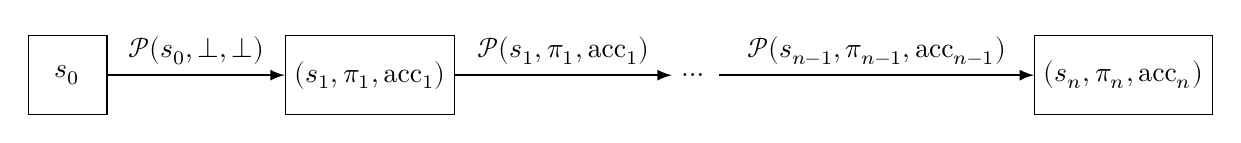
\begin{tikzpicture}[node distance=2.25cm]

  % Nodes
  \node (s0) [node] {$s_0$};
  \node (s1) [node, right=of s0] {$(s_1, \pi_1, \acc_1)$};
  \node (dots) [right=2.75cm of s1] {$\dots$};
  \node (sn) [node, right=4cm of dots] {$(s_n, \pi_n, \acc_n)$};

  % Arrows with labels
  \draw[thick-arrow] (s0) -- node[above] {$\Pc(s_0, \bot, \bot)$} (s1);
  \draw[thick-arrow] (s1) -- node[above] {$\Pc(s_1, \pi_1, \acc_1)$} (dots);
  \draw[thick-arrow] (dots) -- node[above] {$\Pc(s_{n-1}, \pi_{n-1}, \acc_{n-1})$} (sn);

\end{tikzpicture}
\caption{
  A visualization of the relationship between $F, \vec{s}, \vec{\pi}$ and
  $\vec{\acc}$ in an IVC setting using Accumulation Schemes. Where $\Pc$ is
  defined to be $\Pc(s_{i-1}, \pi_{i-1}, \acc_{i-1}) = \IVCProver(s_{i-1},
  \pi_{i-1}, \acc_{i-1}) = \pi_i$, $s_i = F(s_{i-1})$, $\acc_i =
  \ASProver(\vec{q}, \acc_{i-1})$.
}
\end{figure}

Before describing the IVC protocol, we first describe the circuit for
the IVC relation as it's more complex than for the naive SNARK-based
approach. Let:

\begin{itemize}
\tightlist
\item
  \(\pi_{i-1} = \vec{q}, \acc_{i-1}, s_{i-1}\) from the previous
  iteration.
\item
  \(s_i = F(s_{i-1})\)
\item
  \(\acc_i = \ASProver(\vec{q}, \acc_{i-1})\)
\end{itemize}

Giving us the public inputs \(x = \{ R_{IVC}, s_0, s_i, \acc_i \}\) and
witness \(w = \{ s_{i-1}, \pi_{i-1} = \vec{q}, \acc_{i-1} \}\), which
will be used to construct the the IVC circuit \(R_{IVC}\): \[
\begin{aligned}
  x_{i-1} &:= \{ R_{IVC}, s_{i-1}, \acc_{i-1} \} \\
  \Vc_1   &:= \SNARKVerifierFast(R_{IVC}, x_{i-1}, \pi_{i-1}) \meq \top \\
  \Vc_2   &:= \ASVerifier(\pi_{i-1} = \vec{q}, \acc_{i-1}, \acc_i) \meq \top \\
  R_{IVC} &:= \text{I.K } w \text{ s.t. } F(s_{i-1}) \meq s_i \land (s_{i-1} \meq s_0 \lor ( \Vc_1 \land \Vc_2 ) ) \\
\end{aligned}
\]

\begin{figure}[H]
\centering
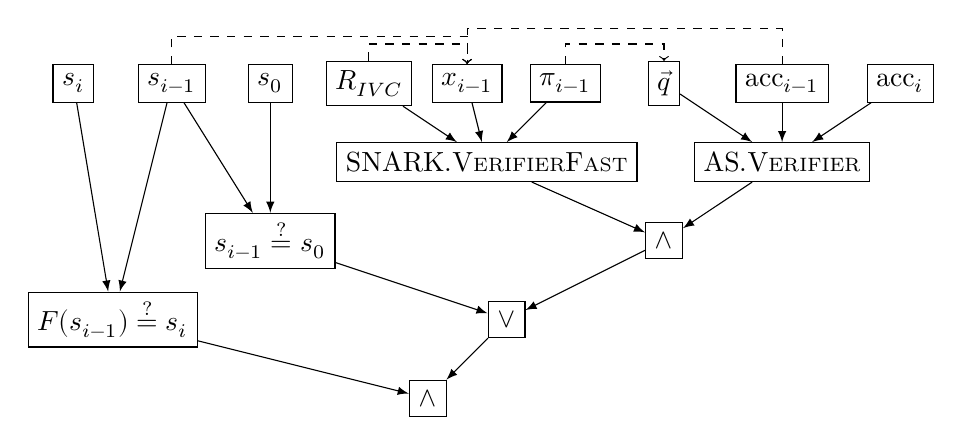
\begin{tikzpicture}
  % First Layer
  \node[draw, rectangle] (q) at (6, 6.5) {$\vec{q}$};
  \node[draw, rectangle] (acc_prev) at (7.5, 6.5) {$\acc_{i-1}$};
  \node[draw, rectangle] (acc_next) at (9, 6.5) {$\acc_i$};

  \node[draw, rectangle] (R_ivc) at (2.25, 6.5) {$R_{IVC}$};
  \node[draw, rectangle] (x_prev) at (3.5, 6.5) {$x_{i-1}$};
  \node[draw, rectangle] (pi_prev) at (4.75, 6.5) {$\pi_{i-1}$};

  \node[draw, rectangle] (s_next) at (-1.5, 6.5) {$s_i$};
  \node[draw, rectangle] (s_prev) at (-0.25, 6.5) {$s_{i-1}$};
  \node[draw, rectangle] (s_0) at (1, 6.5) {$s_0$};

  \draw[dashed-arrow] (pi_prev) -- (4.75, 7) -- (6, 7) -- (q);

  \draw[dashed-arrow] (R_ivc) -- (2.25, 7) -- (3.5, 7) -- (x_prev);
  \draw[dashed-arrow] (s_prev) -- (-0.25, 7.1) -- (3.5, 7.1) -- (x_prev);
  \draw[dashed-arrow] (acc_prev) -- (7.5, 7.2) -- (3.5, 7.2) -- (x_prev);

  % Second Layer
  \node[draw, rectangle] (svf) at (3.75, 5.5) {$\SNARKVerifierFast$};
  \node[draw, rectangle] (asv) at (7.5, 5.5) {$\ASVerifier$};

  \draw[arrow] (R_ivc) -- (svf);
  \draw[arrow] (x_prev) -- (svf);
  \draw[arrow] (pi_prev) -- (svf);

  \draw[arrow] (q) -- (asv);
  \draw[arrow] (acc_prev) -- (asv);
  \draw[arrow] (acc_next) -- (asv);

  % Third Layer
  \node[draw, rectangle] (asv_svf_and) at (6, 4.5) {$\land$};
  \node[draw, rectangle] (base_case) at (1, 4.5) {$s_{i-1} \meq s_0$};

  \draw[arrow] (asv) -- (asv_svf_and);
  \draw[arrow] (svf) -- (asv_svf_and);

  \draw[arrow] (s_prev) -- (base_case);
  \draw[arrow] (s_0) -- (base_case);

  % Fourth Layer
  \node[draw, rectangle] (or) at (4, 3.5) {$\lor$};
  \node[draw, rectangle] (F) at (-1, 3.5) {$F(s_{i-1}) \meq s_i$};

  \draw[arrow] (asv_svf_and) -- (or);
  \draw[arrow] (base_case) -- (or);

  \draw[arrow] (s_next) -- (F);
  \draw[arrow] (s_prev) -- (F);

  % Fifth Layer
  \node[draw, rectangle] (end_and) at (3, 2.5) { $\land$ };
  \draw[arrow] (or) -- (end_and);
  \draw[arrow] (F) -- (end_and);

\end{tikzpicture}
\caption{A visualization of $R_{IVC}$}
\end{figure}

The verifier and prover for the IVC scheme can be seen below:

\begin{algorithm}[H]
\caption*{\textbf{Algorithm} $\IVCProver$}
\textbf{Inputs} \\
  \Desc{$R_{IVC}: \Circuit$}{The IVC circuit as defined above.} \\
  \Desc{$x: \PublicInputs$}{Public inputs for $R_{IVC}$.} \\
  \Desc{$w: \Option(\Witness)$}{Private inputs for $R_{IVC}$.} \\
\textbf{Output} \\
  \Desc{$(S, \Proof, \Acc)$}{The values for the next IVC iteration.}
\begin{algorithmic}[1]
  \Require $x = \{ s_0 \}$
  \Require $w = \{ s_{i-1}, \pi_{i-1}, \acc_{i-1} \} \lor w = \bot$
  \State Parse $s_0$ from $x = \{ s_0 \}$.
  \If{$w = \bot$}
    \State $w = \{ s_{i-1} = s_0 \}$
  \Else
    \State Run the accumulation prover: $\acc_i = \ASProver(\pi_{i-1} = \vec{q}, \acc_{i-1})$.
    \State Compute the next value: $s_i = F(s_{i-1})$.
    \State Augment $x$ with $R_{IVC}, s_i, \acc_i$.
  \EndIf
  \State Then generate a SNARK proof $\pi_i$ using the circuit $R_{IVC}$: $\pi_i = \SNARKProver(R_{IVC}, x, w)$.
  \State Output $(s_i, \pi_i, \acc_i)$
\end{algorithmic}
\end{algorithm}

\begin{algorithm}[H]
\caption*{\textbf{Algorithm} $\IVCVerifier$}
\textbf{Inputs} \\
  \Desc{$R_{IVC}: \Circuit$}{The IVC circuit.} \\
  \Desc{$x: \PublicInputs$}{Public inputs for $R_{IVC}$.} \\
\textbf{Output} \\
  \Desc{$\Result(\top, \bot)$}{Returns $\top$ if the verifier accepts and $\bot$ if the verifier rejects.}
\begin{algorithmic}[1]
  \Require $x = \{ s_0, s_i, \acc_i \}$
  \State Augment $x$ with $R_{IVC}$.
  \State Verify that the accumulation scheme decider accepts: $\top \meq \ASDecider(\acc_i)$.
  \State Verify the validity of the IVC proof: $\top \meq \SNARKVerifier(R_{IVC}, x, \pi_i)$.
  \State If the above two checks pass, then output $\top$, else output $\bot$.
\end{algorithmic}
\end{algorithm}

Consider the above chain run \(n\) times. As in the ``simple'' SNARK IVC
construction, if \(\IVCVerifier\) accepts at the end, then we get a
chain of implications: \[
\begin{alignedat}[b]{2}
  &\IVCVerifier(R_{IVC}, x_n = \{ s_0, s_n, \acc_i \}, \pi_n) = \top           &&\then \\
  &\forall i \in [n], \forall q_j \in \pi_i = \vec{q} : \PCDLCheck(q_j) = \top &&\;\; \land \\
  &F(s_{n-1}) = s_n     \land (s_{n-1} = s_0 \lor ( \Vc_1 \land \Vc_2 ))       &&\then \\
  &\ASVerifier(\pi_{n-1}, \acc_{n-1}, \acc_n)                                  &&\;\; \land \\
  &\SNARKVerifierFast(R_{IVC}, x_{n-1}, \pi_{n-1})                             &&\then \dots \\
  &F(s_0) = s_1 \land (s_0 = s_0 \lor ( \Vc_1 \land \Vc_2 ))                   &&\then \\
  &F(s_0) = s_1                                                                &&\then \\
\end{alignedat}
\] Since \(\IVCVerifier\) runs \(\ASDecider\), the previous accumulator
is valid, and by recursion, all previous accumulators are valid.
Therefore, if a \(\ASVerifier\)'s accept, that means that
\(\vec{q} = \pi_i\) are valid evaluation proofs. We defined
\(\SNARKVerifierFast\), s.t. it verifies correctly provided the
\(\vec{q}\)'s are valid evaluation proofs. This allows us to recurse
through this chain of implications.

From this we learn:

\begin{enumerate}
\def\labelenumi{\arabic{enumi}.}
\tightlist
\item
  \(\forall i \in [2, n] : \ASVerifier(\pi_{i-1}, \acc_{i-1}, \acc_i) = \top\),
  i.e, all accumulators are accumulated correctly.
\item
  \(\forall i \in [2, n] : \SNARKVerifierFast(R_{IVC}, x_{i-1}, \pi_{i-1})\),
  i.e, all the proofs are valid. Giving us our precondition for
  \(\ASDecider\).
\end{enumerate}

These points in turn imply that
\(\forall i \in [n] : F(s_{i-1}) = s_i\), therefore, \(s_n = F^n(s_0)\).
From this discussion it should be clear that an honest prover will
convince an honest verifier, i.e.~completeness holds. As for soundness,
it should mostly depend on the soundness of the underlying PCS,
accumulation scheme and SNARK\footnote{A more thorough soundness
  discussion would reveal that running the extractor on a proof-chain of
  length \(n\) actually fails, as argued by Valiant in his original 2008
  paper. Instead he constructs a proof-tree of size \(\Oc(\lg(n))\)
  size, to circumvent this. However, practical applications conjecture
  that the failure of the extractor does not lead to any real-world
  attack, thus still achieving constant proof sizes, but with an
  additional security assumption added.}.

As for efficiency, assuming that:

\begin{itemize}
\tightlist
\item
  The runtime of \(\SNARKProver\) scales linearly with the degree-bound,
  \(d\), of the polynomial, \(p_j\), used for each \(q_j \in \vec{q}_m\)
  (\(\Oc(d)\))
\item
  The runtime of \(\SNARKVerifierFast\) scales logarithmically with the
  degree-bound, \(d\), of \(p_j\) (\(\Oc(\lg(d))\))
\item
  The runtime of \(\SNARKVerifier\) scales linearly with the
  degree-bound, \(d\), of \(p_j\) (\(\Oc(d)\))
\item
  The runtime of \(F\) is less than \(\Oc(d)\), since it needs to be
  compiled to a circuit of size at most \(\approx d\)
\end{itemize}

Then we can conclude:

\begin{itemize}
\tightlist
\item
  The runtime of \(\IVCProver\) is:

  \begin{itemize}
  \tightlist
  \item
    Step 5: The cost of running \(\ASDLProver\), \(\Oc(d)\).
  \item
    Step 6: The cost of computing \(F\), \(\Oc(F(x))\).
  \item
    Step 7: The cost of running \(\SNARKProver\), \(\Oc(d)\).
  \end{itemize}

  Totalling \(\Oc(F(x) + d)\). So \(\Oc(d)\).
\item
  The runtime of \(\IVCVerifier\) is:

  \begin{itemize}
  \tightlist
  \item
    Step 2: The cost of running \(\ASDLDecider\), \(\Oc(d)\) scalar
    multiplications.
  \item
    Step 3: The cost of running \(\SNARKVerifier\), \(\Oc(d)\) scalar
    multiplications.
  \end{itemize}

  Totalling \(\Oc(2d)\). So \(\Oc(d)\)
\end{itemize}

Notice that although the runtime of \(\IVCVerifier\) is linear, it
scales with \(d\), \emph{not} \(n\). So the cost of verifying does not
scale with the number of iterations.

\subsection{The Implementation}\label{the-implementation}

The authors of the accumulation scheme paper{[}\citeproc{ref-pcd}{Bünz
et al. 2020}{]} also define a concrete Accumulation Scheme using the
Discrete Log assumption \(\ASDL\), which uses the same algorithms as in
the 2019 Halo paper. This accumulation scheme in turn, relies heavily
upon a Polynomial Commitment Scheme, \(\PCDL\), which is also described
in the paper. Both of these have been implemented as part of this
project in Rust and the rest of the document will go over these sets of
algorithms, their security, performance and implementation details.

Since these kinds of proofs can both be used for proving knowledge of a
large witness to a statement succinctly, and doing so without revealing
any information about the underlying witness, the zero-knowledge
property of the protocol is described as \emph{optional}. This is
highlighted in the algorithmic specifications as the parts colored
\textblue{blue}. In the Rust implementation these parts were included as
they were not too cumbersome to implement. However, since the motivation
for this project was IVC, wherein the primary focus is succinctness, not
zero-knowledge, the zero-knowledge parts of the protocol have been
omitted from the soundness, completeness and efficiency discussions.

The authors of the paper present additional algorithms for distributing
public parameters (\(\CMTrim\), \(\PCDLTrim\), \(\ASDLIndexer\)), we
omit them in the following algorithmic specifications on the assumption
that:

\begin{enumerate}
\def\labelenumi{\alph{enumi}.}
\tightlist
\item
  The setups has already been run, producing values
  \(N, D \in \Nb, S, H \in_R
  \Eb(\Fb_q), \vec{G} \in_R \Eb(\Fb_q)\) where \(D = N - 1\), \(N\) is a
  power of two and any random values have been sampled honestly.
\item
  All algorithms have global access to the above values.
\end{enumerate}

This closely models the implementation where the public parameters were
randomly sampled using a hashing algorithm for a computationally viable
value of \(N\). As described in the subsection on trusted and untrusted
setups, a genesis string was prepended with an numeric index, run
through the sha3 hashing algorithm, then used to generate curve points.
These must be generators for \(\Eb(\Fb_q)\) but since all points (except
the identity point \(\Oc\)) of the Pallas curve used are generators,
they were simply sampled uniformly randomly from all of \(\Eb(\Fb_q)\).
These values were then added as global constants in the code. See the
\href{https://github.com/rasmus-kirk/halo-accumulation/blob/main/code/src/consts.rs}{\texttt{/code/src/consts.rs}}
in the repository for more details. The associated rust code for
generating the public parameters can be seen below:

\begin{Shaded}
\begin{Highlighting}[numbers=left,,]
\KeywordTok{fn}\NormalTok{ get\_urs\_element(i}\OperatorTok{:} \DataTypeTok{usize}\NormalTok{) }\OperatorTok{{-}\textgreater{}}\NormalTok{ PallasPoint }\OperatorTok{\{}
    \KeywordTok{let}\NormalTok{ genesis\_string }\OperatorTok{=} \StringTok{"To understand recursion, one must first understand recursion"}\OperatorTok{;}

    \CommentTok{// Hash \textasciigrave{}i\textasciigrave{} concatenated with \textasciigrave{}genesis\_string\textasciigrave{}}
    \KeywordTok{let} \KeywordTok{mut}\NormalTok{ hasher }\OperatorTok{=} \PreprocessorTok{Sha3\_256::}\NormalTok{new()}\OperatorTok{;}
\NormalTok{    hasher}\OperatorTok{.}\NormalTok{update(i}\OperatorTok{.}\NormalTok{to\_le\_bytes())}\OperatorTok{;}
\NormalTok{    hasher}\OperatorTok{.}\NormalTok{update(genesis\_string}\OperatorTok{.}\NormalTok{as\_bytes())}\OperatorTok{;}
    \KeywordTok{let}\NormalTok{ hash\_result }\OperatorTok{=}\NormalTok{ hasher}\OperatorTok{.}\NormalTok{finalize()}\OperatorTok{;}

    \PreprocessorTok{PallasPoint::}\NormalTok{generator() }\OperatorTok{*} \PreprocessorTok{PallasScalar::}\NormalTok{from\_le\_bytes\_mod\_order(}\OperatorTok{\&}\NormalTok{hash\_result)}
\OperatorTok{\}}
\KeywordTok{fn}\NormalTok{ get\_pp(n}\OperatorTok{:} \DataTypeTok{usize}\NormalTok{) }\OperatorTok{{-}\textgreater{}}\NormalTok{ (PallasPoint}\OperatorTok{,}\NormalTok{ PallasPoint}\OperatorTok{,} \DataTypeTok{Vec}\OperatorTok{\textless{}}\NormalTok{PallasPoint}\OperatorTok{\textgreater{}}\NormalTok{) }\OperatorTok{\{}
    \KeywordTok{let}\NormalTok{ S }\OperatorTok{=}\NormalTok{ get\_urs\_element(}\DecValTok{0}\NormalTok{)}\OperatorTok{;}
    \KeywordTok{let}\NormalTok{ H }\OperatorTok{=}\NormalTok{ get\_urs\_element(}\DecValTok{1}\NormalTok{)}\OperatorTok{;}
    \KeywordTok{let} \KeywordTok{mut}\NormalTok{ Gs }\OperatorTok{=} \DataTypeTok{Vec}\PreprocessorTok{::}\NormalTok{with\_capacity(n)}\OperatorTok{;}
    \ControlFlowTok{for}\NormalTok{ i }\KeywordTok{in} \DecValTok{2}\OperatorTok{..}\NormalTok{(n }\OperatorTok{+} \DecValTok{2}\NormalTok{) }\OperatorTok{\{}
\NormalTok{        Gs}\OperatorTok{.}\NormalTok{push(get\_urs\_element(i))}
    \OperatorTok{\}}
\NormalTok{    (S}\OperatorTok{,}\NormalTok{ H}\OperatorTok{,}\NormalTok{ Gs)}
\OperatorTok{\}}
\end{Highlighting}
\end{Shaded}

\newpage

\section{\texorpdfstring{\(\PCDL\): The Polynomial Commitment
Scheme}{\textbackslash PCDL: The Polynomial Commitment Scheme}}\label{pcdl-the-polynomial-commitment-scheme}

\subsection{Outline}\label{outline}

The Polynomial Commitment Scheme, \(\PCDL\), is based on the discrete
log assumption, and does not require a Trusted Setup. Most of the
functions simply works as one would expect for a PCS, but uniquely for
this scheme, we have the function \(\PCDLSuccinctCheck\) that allows
deferring the expensive part of checking PCS openings until a later
point. This function is what leads to the accumulation scheme based on
the discrete log assumption \(\ASDL\). We have five main functions:

\begin{itemize}
\item
  \(\PCDLSetup(\l, D)^{\rho_0} \to \pp_\PC\)

  The setup routine. Given security parameter \(\l\) in unary and a
  maximum degree bound \(D\):

  \begin{itemize}
  \tightlist
  \item
    Runs \(\pp_\CM \from \CMSetup(\l, D + 1)\),
  \item
    Samples \(H \in \Eb(\Fb_q)\) using the random oracle
    \(H \from \rho_0(\pp_\CM)\),
  \item
    Finally, outputs \(\pp_\PC = (\pp_\CM, H)\).
  \end{itemize}
\item
  \(\PCDLCommit(p: \Fb^d_q[X]{, \o: \Option(\Fb_q)}) \to \Eb(\Fb_q)\):

  Creates a commitment to the coefficients of the polynomial \(p\) of
  degree \(d\) with optional hiding \(\o\), using Pedersen commitments.
\item
  \(\PCDLOpen^{\rho_0}(p: \Fb^d_q[X], C: \Eb(\Fb_q), z: \Fb_q\mathblue{, \o: \Option(\Fb_q)}) \to \EvalProof\):

  Creates a proof \(\pi\) that states: ``I know \(p \in \Fb^d_q[X]\)
  with commitment \(C \in \Eb(\Fb_q)\) s.t. \(p(z) = v\)'' where \(p\)
  is private and \(d, z, v\) are public.
\item
  \(\PCDLSuccinctCheck^{\rho_0}(C: \Eb(\Fb_q), d: \Nb, z: \Fb_q, v: \Fb_q, \pi: \EvalProof) \to \Result((\Fb^d_q[X], \Gb), \bot)\):

  Cheaply checks that a proof \(\pi\) is correct. It is not a full check
  however, since an expensive part of the check is deferred until a
  later point.
\item
  \(\PCDLCheck^{\rho_0}(C: \Eb(\Fb_q), d: \Nb, z: \Fb_q, v: \Fb_q, \pi: \EvalProof) \to \Result(\top, \bot)\):

  The full check on \(\pi\).
\end{itemize}

The following subsections will describe them in pseudo-code, except for
\(\PCDLSetup\).

\subsubsection{\texorpdfstring{\(\PCDLCommit\)}{\textbackslash PCDLCommit}}\label{pcdlcommit}

\begin{algorithm}[H]
\caption{$\PCDLCommit$}
\textbf{Inputs} \\
  \Desc{$p: \Fb^d_q[X]$}{The univariate polynomial that we wish to commit to.} \\
  \Desc{$\mathblue{\o: \Option(\Fb_q)}$}{Optional hiding factor for the commitment.} \\
\textbf{Output} \\
  \Desc{$C: \Eb(\Fb_q)$}{The Pedersen commitment to the coefficients of polynomial $p$.}
\begin{algorithmic}[1]
  \Require $d \leq D$
  \Require $(d+1)$ is a power of 2.
  \State Let $\vec{p}$ be the coefficient vector for $p$
  \State Output $C := \CMCommit(\vec{G}, \vec{p}, \mathblue{\o})$.
\end{algorithmic}
\end{algorithm}

\(\PCDLCommit\) is rather simple, we just take the coefficients of the
polynomial and commit to them using a Pedersen commitment.

\subsubsection{\texorpdfstring{\(\PCDLOpen\)}{\textbackslash PCDLOpen}}\label{pcdlopen}

\begin{algorithm}[H]
\caption{$\PCDLOpen^{\rho_0}$}
\textbf{Inputs} \\
  \Desc{$p: \Fb^d_q[X]$}{The univariate polynomial that we wish to open for.} \\
  \Desc{$C: \Eb(\Fb_q$)}{A commitment to the coefficients of $p$.} \\
  \Desc{$z: \Fb_q$}{The element that $z$ will be evaluated on $v = p(z)$.} \\
  \Desc{$\mathblue{\o: \Option(\Fb_q)}$}{Optional hiding factor for $C$. \textit{Must} be included if $C$ was created with hiding!} \\
\textbf{Output} \\
  \Desc{$\EvalProof$}{
    Proof that states: "I know $p \in \Fb^d_q[X]$ with commitment $C \in
    \Eb(\Fb_q)$ s.t. $p(z) = v$"
  }
\begin{algorithmic}[1]
  \Require $d \leq D$
  \Require $(d+1)$ is a power of 2.
  \State Let $n = d+1$
  \State Compute $v = p(z)$ and let $n = d+1$.
  \State \textblue{Sample a random polynomial $\bar{p} \in \Fb^{\leq d}_q[X]$ such that $\bar{p}(z) = 0$}.
  \State \textblue{Sample corresponding commitment randomness $\bar{\o} \in \Fb_q$.}
  \State \textblue{Compute a hiding commitment to $\bar{p}$: $\bar{C} \gets \CMCommit(\vec{G}, \bar{p}, \bar{\o}) \in \Gb$.}
  \State \textblue{Compute the challenge $\a := \rho_0(C, z, v, \bar{C}) \in \Fb^{*}_q$.}
  \State \textblue{Compute commitment randomness $\o' := \o + \a \bar{\o} \in \Fb_q$}.
  \State Compute the polynomial $p' := p \mathblue{+ \a \bar{p}} = \sum_{i=0} c_i X_i \in \Fb_q[X]$.
  \State Compute a non-hiding commitment to $p'$: $C' := C \mathblue{+ \a \bar{C} - \o' S} \in \Gb$.
  \State Compute the 0-th challenge field element $\xi_0 := \rho_0(C', z, v) \in \Fb_q$, then $H' := \xi_0 H \in \Gb$.
  \State Initialize the vectors ($\vec{c_0}$ is defined to be coefficient vector of $p'$):
    \Statex \algind $
      \begin{alignedat}[b]{1}
        \vec{c_0} &:= (c_0, c_1, \dots, c_d) \in F^n_q \\ 
        \vec{z_0} &:= (1, z^1, \dots, z^d) \in F^n_q \\
        \vec{G_0} &:= (G_0, G_1, \dots, G_d) \in \Gb_n \\
      \end{alignedat}
    $
  \For{$i \in [\lg(n)]$}
    \State Compute $L_i := \CMCommit(l(\vec{G_{i-1}}) \cat H', \; \;  r(\vec{c_{i-1}}) \cat \langle r(\vec{c_{i-1}}), l(\vec{z_{i-1}}) \rangle, \; \; \bot)$
    \State Compute $R_i := \CMCommit(r(\vec{G_{i-1}}) \cat H', \; \; l(\vec{c_{i-1}}) \cat \langle l(\vec{c_{i-1}}), r(\vec{z_{i-1}}) \rangle, \; \; \bot)$
    \State Generate the i-th challenge $\xi_i := \rho_0(\xi_{i-1}, L_i, R_i) \in \Fb_q$.
    \State Construct commitment inputs for the next round: 
      \Statex \algindd $
        \begin{alignedat}[b]{3}
          \vec{G_i} &:= l(\vec{G_{i-1}}) &&+ \xi_i      &&\cdot r(\vec{G_{i-1}}) \\ 
          \vec{c_i} &:= l(\vec{c_{i-1}}) &&+ \xi^{-1}_i &&\cdot r(\vec{c_{i-1}}) \\
          \vec{z_i} &:= l(\vec{z_{i-1}}) &&+ \xi_i      &&\cdot r(\vec{z_{i-1}}) \\
        \end{alignedat}
      $
  \EndFor
  \State Finally output the evaluation proof $\pi := (\vec{L},\vec{R}, U := G^{(0)}, c := c^{(0)}, \mathblue{\bar{C}, \o'})$
\end{algorithmic}
\end{algorithm}

The \(\PCDLOpen\) algorithm mostly follows the IPA algorithm from
Bulletproofs. Except,in this case we are trying to prove we know
polynomial \(p\) s.t. \(p(z) = v = \dotp{\vec{c_0}}{\vec{z_0}}\). So
because \(z\) is public, we can get away with omitting the generators,
\((\vec{H})\), for \(\vec{b}\) which we would otherwise need in the
Bulletproofs IPA. For efficiency we also send along the curve point
\(U = G^{(0)}\), which the original IPA does not do. The
\(\PCDLSuccinctCheck\) uses \(U\) to make its check and \(\PCDLCheck\)
verifies the correctness of \(U\).

\subsubsection{\texorpdfstring{\(\PCDLSuccinctCheck\)}{\textbackslash PCDLSuccinctCheck}}\label{pcdlsuccinctcheck}

\begin{algorithm}[H]
\caption{$\PCDLSuccinctCheck^{\rho_0}$}
\textbf{Inputs} \\
  \Desc{$C: \Eb(\Fb_q)$}{A commitment to the coefficients of $p$.} \\
  \Desc{$d: \Nb$}{A degree bound on $p$} \\
  \Desc{$z: \Fb_q$}{The element that $p$ is evaluated on.} \\
  \Desc{$v: \Fb_q$}{The claimed element $v = p(z)$.} \\
  \Desc{$\pi: \EvalProof$}{The evaluation proof produced by $\PCDLOpen$} \\
\textbf{Output} \\
  \Desc{$\Result((\Fb^d_q[X], \Gb), \bot)$}{
    The algorithm will either succeed and output ($h: \Fb^d_q[X], U: \Gb$) if $\pi$ is a valid proof and otherwise fail ($\bot$).
  }
\begin{algorithmic}[1]
  \Require $d \leq D$
  \Require $(d+1)$ is a power of 2.
  \State Parse $\pi$ as $(\vec{L},\vec{R}, U := G^{(0)}, c := c^{(0)}, \mathblue{\bar{C}, \o'})$ and let $n = d + 1$.
  \State \textblue{Compute the challenge $\alpha := \rho_0(C, z, v, \bar{C}) \in F^{*}_q$.}
  \State Compute the non-hiding commitment $C' := C \mathblue{+ \a \bar{C} - \o'S} \in \Gb$.
  \State Compute the 0-th challenge: $\xi_0 := \rho_0(C', z, v)$, and set $H' := \xi_0 H \in \Gb$.
  \State Compute the group element $C_0 := C' + vH' \in \Gb$.
  \For{$i \in [\lg(n)]$}
    \State Generate the i-th challenge: $\xi_i := \rho_0(\xi_{i-1}, L_i, R_i) \in \Fb_q$.
    \State Compute the i-th commitment: $C_i := \xi^{-1}_i L_i + C_{i-1} + \xi_i R_i \in \Gb$.
  \EndFor
\State Define the univariate polynomial $h(X) := \prod^{\lg(n)-1}_{i=0} (1 + \xi_{\lg(n) - i} X^{2^i}) \in \Fb_q[X]$.
\State Compute the evaluation $v' := c \cdot h(z) \in \Fb_q$.
\State Check that $C_{lg(n)} \meq cU + v'H'$
\State Output $(h(X), U)$.
\end{algorithmic}
\end{algorithm}

The \(\PCDLSuccinctCheck\) algorithm performs the same check as in the
Bulletproofs protocol. With the only difference being that instead of
calculating \(G^{(0)}\) itself, it trusts that the verifier sent the
correct \(U
= G^{(0)}\) in the prover protocol, and defers the verification of this
claim to \(\PCDLCheck\). Notice also the ``magic'' polynomial \(h(X)\),
which has a degree \(d\), but can be evaluated in \(\lg(d)\) time.

\subsubsection{\texorpdfstring{\(\PCDLCheck\)}{\textbackslash PCDLCheck}}\label{pcdlcheck}

\begin{algorithm}[H]
\caption{$\PCDLCheck^{\rho_0}$}\label{alg:pcdl_check}
\textbf{Inputs} \\
  \Desc{$C: \Eb(\Fb_q)$}{A commitment to the coefficients of $p$.} \\
  \Desc{$d: \Nb$}{A degree bound on $p$} \\
  \Desc{$z: \Fb_q$}{The element that $p$ is evaluated on.} \\
  \Desc{$v: \Fb_q$}{The claimed element $v = p(z)$.} \\
  \Desc{$\pi: \EvalProof$}{The evaluation proof produced by $\PCDLOpen$} \\
\textbf{Output} \\
  \Desc{$\Result(\top, \bot)$}{The algorithm will either succeed ($\top$) if $\pi$ is a valid proof and otherwise fail ($\bot$).}
\begin{algorithmic}[1]
  \Require $d \leq D$
  \Require $(d+1)$ is a power of 2.
  \State Check that $\PCDLSuccinctCheck(C, d, z, v, \pi)$ accepts and outputs $(h, U)$.
  \State Check that $U \meq \CMCommit(\vec{G}, \vec{h}^{\text{(coeffs)}}, \bot)$, where $\vec{h}^{\text{(coeffs)}}$ is the coefficient vector of the polynomial $h$.
\end{algorithmic}
\end{algorithm}

Since \(\PCDLSuccinctCheck\) handles the verification of the IPA given
that \(U = G^{(0)}\), we run \(\PCDLSuccinctCheck\), then check that
\(U \meq (G^{(0)}
= \CMCommit(\vec{G}, \vec{h}^{\text{(coeffs)}}, \bot) = \ip{\vec{G}}{\vec{h}^{\text{(coeffs)}}})\).

\subsection{Completeness}\label{completeness}

\textbf{Check 1} (\(C_{lg(n)} \meq cU + v'H'\)) \textbf{in
\(\PCDLSuccinctCheck\):}

Let's start by looking at \(C_{lg(n)}\). The verifier computes
\(C_{lg(n)}\) as: \[
\begin{aligned}
  C_0        &= C' + vH' = C + vH' \\
  C_{\lg(n)} &= C_0 + \sum^{\lg(n)-1}_{i=0} \xi^{-1}_{i+1} L_i + \xi_{i+1} R_i \\
\end{aligned}
\] Given that the prover is honest, the following invariant should hold:
\[
\begin{alignedat}[b]{1}
  C_{i+1} &= \ip{\vec{c}_{i+1}}{\vec{G}_{i+1}} + \ip{\vec{c}_{i+1}}{\vec{z}_{i+1}} H'\\ 
          &= \ip{l(\vec{c}_i) + \xi^{-1}_{i+1} r(\vec{c}_i)}{l(\vec{G}_i) + \xi_{i+1} r(\vec{G}_i)} 
            + \ip{l(\vec{c}_i) + \xi^{-1}_{i+1} r(\vec{c}_i)}{l(\vec{z}_i) + \xi_{i+1} r(\vec{z}_i)} H'\\
          &= \ip{l(\vec{c}_i)}{l(\vec{G}_i)} + \xi_{i+1} \ip{l(\vec{c}_i))}{r(\vec{G}_i}
            + \xi^{-1}_{i+1} \ip{r(\vec{c}_i)}{l(\vec{G}_i)} + \ip{r(\vec{c}_i)}{r(\vec{G}_i)}\\
          &+ (\ip{l(\vec{c}_i)}{l(\vec{z}_i)} + \xi_{i+1} \ip{l(\vec{c}_i)}{r(\vec{z}_i)} 
            + \xi^{-1}_{i+1} \ip{r(\vec{c}_i)}{l(\vec{z}_i)} + \ip{r(\vec{c}_i)}{l(\vec{z}_i)}) H'
\end{alignedat}
\] If we group these terms: \[
\begin{alignedat}[b]{4}
  C_{i+1} &= \ip{l(\vec{c}_i)}{l(\vec{z}_i)}  &&+ \ip{r(\vec{c}_i)}{r(\vec{G}_i)}     &&+ \xi_{i+1} \ip{l(\vec{c}_i)}{r(\vec{G}_i)}    &&+ \xi^{-1}_{i+1} \ip{r(\vec{c}_i)}{l(\vec{G}_i)} \\
          &+ (\ip{l(\vec{c}_i)}{l(\vec{z}_i)} &&+ \ip{r(\vec{c}_i)}{r(\vec{z}_i)}) H' &&+ \xi_{i+1} \ip{l(\vec{c}_i)}{r(\vec{z}_i)} H' &&+ \xi^{-1}_{i+1} \ip{r(\vec{c}_i)}{l(\vec{z}_i)} H' \\
          &= C_i                              &&                                      &&+ \xi_{i+1} R_i                                &&+ \xi^{-1}_{i+1} L_i \\
          &\mkern-18mu\mkern-18mu \textbf{Where:} && && && \\
  L_i     &= \ip{r(\vec{c}_i)}{l(\vec{G}_i)} &&+ \ip{r(\vec{c}_i)}{l(\vec{z}_i)} H' && && \\
  R_i     &= \ip{l(\vec{c}_i)}{r(\vec{G}_i)} &&+ \ip{l(\vec{c}_i)}{r(\vec{z}_i)} H' && && 
\end{alignedat}
\] We see why \(\vec{L}, \vec{R}\) is defined the way they are. They
help the verifier check that the original relation hold, by showing it
for the compressed form \(C_{i+1}\). \(\vec{L}, \vec{R}\) is just the
minimal information needed to communicate this fact.

This leaves us with the following vectors (notice the slight difference
in length): \[
\begin{alignedat}[b]{1}
  \vec{L}    &= (L_1, \dots, L_{\lg(n)}) \\
  \vec{R}    &= (R_1, \dots, R_{\lg(n)}) \\
  \vec{C}    &= (C_0, \dots, C_{\lg(n)}) \\
  \vec{\xi}  &= (\xi_0, \dots, \xi_{\lg(n)}) \\
\end{alignedat}
\] This means an honest prover will indeed produce \(\vec{L}, \vec{R}\)
s.t.
\(C_{\lg(n)} = C_0 + \sum^{\lg(n)-1}_{i=0} \xi^{-1}_{i+1} L_i + \xi_{i+1}
R_i\)

Let's finally look at the left-hand side of the verifying check:

\[C_{\lg(n)} = C_0 + \sum^{\lg(n)-1}_{i=0} \xi^{-1}_{i+1} L_i + \xi_{i+1} R_i\]
The original definition of \(C_i\):
\[C_{\lg(n)} = \ip{\vec{c}_{\lg(n)}}{\vec{G}_{\lg(n)}} + \ip{\vec{c}_{\lg(n)}}{\vec{z}_{\lg(n)}} H'\]
Vectors have length one, so we use the single elements
\(c^{(0)}, G^{(0)}, c^{(0)}, z^{(0)}\) of the vectors:
\[C_{\lg(n)} = c^{(0)}G^{(0)} + c^{(0)}z^{(0)} H'\] The verifier has
\(c^{(0)} = c, G^{(0)} = U\) from \(\pi \in \EvalProof\):
\[C_{\lg(n)} = cU + cz^{(0)} H'\] Then, by construction of
\(h(X) \in \Fb^d_q[X]\): \[C_{\lg(n)} = cU + ch(z) H'\] Finally we use
the definition of \(v'\): \[C_{\lg(n)} = cU + v'H'\]

Which corresponds exactly to the check that the verifier makes.

\textbf{Check 2}
(\(U \meq \CMCommit(\vec{G}, \vec{h}^{\text{(coeffs)}}, \bot)\))
\textbf{in \(\PCDLCheck\):}

The honest prover will define \(U = G^{(0)}\) as promised and the
right-hand side will also become \(U = G^{(0)}\) by the construction of
\(h(X)\).

\subsection{Knowledge Soundness}\label{knowledge-soundness}

This subsection will not contain a full knowledge soundness proof, but
it will be briefly argued that the \emph{non-zero-knowledge} version of
\(\PCDL\) should be knowledge sound. The knowledge soundness property of
\(\PCDL\) states: \[
\Pr \left[
  \begin{array}{c}
    \PCCheck^\rho(C, d, z, v, \pi) = 1 \\
    \Downarrow \\
    C = \PCCommit^\rho(p, d, \o) \\
    v = p(z), \; \deg(p) \leq d \leq D
  \end{array}
  \middle|
  \begin{array}{r}
    \rho \leftarrow \Uc(\l) \\
    \pp_\PC \leftarrow \PCSetup^\rho(1^\l, D) \\
    (C, d, z, v, \pi) \leftarrow \Ac^\rho(\pp_\PC) \\
    (p, \o) \leftarrow \Ec^\rho(\pp_\PC) \\
  \end{array}
\right] \geq 1 - \negl(\lambda).
\] So, we need to show that:

\begin{enumerate}
\def\labelenumi{\arabic{enumi}.}
\tightlist
\item
  \(C = \PCCommit^\rho(p, d, \o)\)
\item
  \(v = p(z)\)
\item
  \(\deg(p) \leq d \leq D\)
\end{enumerate}

The knowledge extractability of \(\PCDL\) is almost identical to the IPA
from bulletproofs{[}\citeproc{ref-bulletproofs}{Bünz et al. 2017}{]}, so
we assume that we can use the same extractor\footnote{Admittedly, this
  assumption is not a very solid one if the purpose was to create a
  proper knowledge soundness proof, but as the section is more-so
  devoted to give a justification for why \(\PCDL\) \emph{ought to be}
  sound, it will do. In fact, the authors of the accumulation scheme
  paper{[}\citeproc{ref-pcd}{Bünz et al. 2020}{]}, use a similar
  argument more formally by stating (without direct proof!), that the
  \(\PCDL\) protocol is a special case of the IPA presented in another
  paper{[}\citeproc{ref-ipa}{Bünz et al. 2019}{]} by mostly the same
  authors.}, with only minor modifications. The IPA extractor extracts
\(\vec{a}, \vec{b} \in \Fb_q^n\) s.t:
\[P = \ip{\vec{G}}{\vec{a}} + \ip{\vec{H}}{\vec{b}} \land v = \ip{\vec{c}}{\vec{z}}\]
Running the extractor for \(\PCDL\) should yield:
\[P = \ip{\vec{G}}{\vec{c}} + \ip{\vec{G}}{\vec{z}} \land v = \ip{\vec{c}}{\vec{z}}\]
We should be able to remove the extraction of \(\vec{z}\) since it's
public: \[C = \ip{\vec{G}}{\vec{c}} \land v = \ip{\vec{c}}{\vec{z}}\]

\begin{enumerate}
\def\labelenumi{\arabic{enumi}.}
\tightlist
\item
  \(C = \ip{\vec{G}}{\vec{c}} = \PCCommit(c, G, \bot) = \PCCommit^\rho(p,
  d, \bot)\), \(\o = \bot\) since we don't consider zero-knowledge.
\item
  \(v = \ip{\vec{c}}{\vec{z}} = \ip{\vec{p}^{\text{(coeffs)}}}{\vec{z}} =
  p(z)\) by definition of \(p\).
\item
  \(\deg(p) \leq d \leq D\). The first bound holds since the vector
  committed to is known to have length \(n = d+1\), the second bound
  holds trivially, as it's checked by \(\PCDLCheck\)
\end{enumerate}

The authors, of the paper followed{[}\citeproc{ref-pcd}{Bünz et al.
2020}{]}, note that the soundness technically breaks down when turning
the IPA into a non-interactive protocol (which is the case for
\(\PCDL\)), and that transforming the IPA into a non-interactive
protocol such that the knowledge extractor does not break down is an
open problem:

\begin{quote}
\color{GbGrey}

\textbf{Security of the resulting non-interactive argument.} It is known
from folklore that applying the Fiat–Shamir transformation to a public-coin
$k$-round interactive argument of knowledge with negligible soundness error
yields a non-interactive argument of knowledge in the random-oracle model
where the extractor $\Ec$ runs in time exponential in $k$. In more detail, to
extract from an adversary that makes $t$ queries to the random oracle, $\Ec$
runs in time $t^{\Oc(k)}$. In our setting, the inner-product argument has $k
= \Oc(\log d)$ rounds, which means that if we apply this folklore result, we
would obtain an extractor that runs in superpolynomial (but sub-exponential)
time $t^{\Oc(\log d)} = 2^{\Oc(log(\l)^2)}$. It remains an interesting open
problem to construct an extractor that runs in polynomial time.

\end{quote}

This has since been solved in a 2023
paper{[}\citeproc{ref-attema}{Attema et al. 2023}{]}. The abstract of
the paper describes:

\begin{quote}
\color{GbGrey}

Unfortunately, the security loss for a $(2\mu + 1)$-move protocol is, in
general, approximately $Q^\mu$, where $Q$ is the number of oracle queries
performed by the attacker. In general, this is the best one can hope for,
as it is easy to see that this loss applies to the $\mu$-fold sequential
repetition of $\Sigma$-protocols, $\dots$, we show that for $(k^1, \dots,
k^\mu)$-special-sound protocols (which cover a broad class of use cases),
the knowledge error degrades linearly in $Q$, instead of $Q^\mu$.

\end{quote}

The IPA is exactly such a \((k^1, \dots,k^\mu)\)-special-sound protocol,
they even directly state that this result applies to bulletproofs. As
such we get a knowledge error that degrades linearly, instead of
superpolynomially, in number of queries, \(t\), that the adversary makes
to the random oracle. As such, the extractor runs in the required
polynomial time (\(\Oc(t) = \Oc(\poly(\l))\)).

\subsection{Efficiency}\label{efficiency}

Given two operations \(f(x), g(x)\) where \(f(x)\) is more expensive
than \(g(x)\), we only consider \(f(x)\), since
\(\Oc(f(n) + g(n)) = \Oc (f(n))\). For all the algorithms, the most
expensive operations will be scalar multiplications. We also don't
bother counting constant operations, that does not scale with the input.
Also note that: \[
  \Oc\left(\sum_{i=2}^{\lg(n)} \frac{n}{i^2}\right) = \Oc\left(n \sum_{i=2}^{\lg(n)} \frac{1}{i^2}\right)
                                       = \Oc(n \cdot c)
                                       = \Oc(n)
\] Remember that in the below contexts \(n = d+1\)

\begin{itemize}
\tightlist
\item
  \(\PCDLCommit\): \(n = \Oc(d)\) scalar multiplications and
  \(n = \Oc(d)\) point additions.
\item
  \(\PCDLOpen\):

  \begin{itemize}
  \tightlist
  \item
    Step 1: 1 polynomial evaluation, i.e.~\(n = \Oc(d)\) field
    multiplications.
  \item
    Step 13 \& 14: Both commit \(\lg(n)\) times,
    i.e.~\(2 (\sum_{i=2}^{\lg(n)} (n+1)/i) = \Oc(2n)\) scalar
    multiplications. The sum appears since we halve the vector length
    each loop iteration.
  \item
    Step 16: \(\lg(n)\) vector dot products,
    i.e.~\(\sum_{i=2}^{\lg(n)} n/i = \Oc(n)\) scalar multiplications.
  \end{itemize}

  In total, \(\Oc(3d)\) scalar multiplications.
\item
  \(\PCDLSuccinctCheck\):

  \begin{itemize}
  \tightlist
  \item
    Step 7: \(\lg(n)\) hashes.
  \item
    Step 8: \(3 \lg(n)\) point additions and \(2 \lg(n)\) scalar
    multiplications.
  \item
    step 11: The evaluation of \(h(X)\) which takes \(\Oc(\lg(n))\)
    time.
  \end{itemize}

  In total, \(\Oc(2 \lg(n)) = \Oc(2 \lg(d))\) scalar multiplications.
\item
  \(\PCDLCheck\):

  \begin{itemize}
  \tightlist
  \item
    Step 1: Running \(\PCDLSuccinctCheck\) takes \(\Oc(2 \lg(d))\)
    scalar multiplications.
  \item
    Step 2: Running
    \(\CMCommit(\vec{G}, \vec{h}^{\text{(coeffs)}}, \bot)\) takes
    \(\Oc(d)\) scalar multiplications.
  \end{itemize}

  Since step two dominates, we have \(\Oc(d)\) scalar multiplications.
\end{itemize}

So \(\PCDLOpen\), \(\PCDLCheck\) and \(\PCDLCommit\) is linear and,
importantly, \(\PCDLSuccinctCheck\) is sub-linear.

\begin{quote}
\color{GbGrey}

\textbf{Sidenote: The runtime of $h(X)$}

Recall the structure of $h(X)$:
$$h(X) := \prod^{\lg(n)-1}_{i=0} (1 + \xi_{\lg(n) - i} X^{2^i}) \in \Fb_q[X]$$
First note that $\prod^{\lg(n)-1}_{i=0} a$ leads to $\lg(n)$
factors. Calculating $X^{2^i}$ can be computed as:
$$X^{2^0}, X^{2^1} = (X^{2^0})^2, X^{2^2} = (X^{2^1})^2$$
So that part of the evaluation boils down to the cost of squaring in the
field. We therefore have $\lg(n)$ squarings (from $X^{2^i}$), and $\lg(n)$
field multiplications from $\xi_{\lg(n) - i} \cdot X^{2^i}$. Each squaring
can naively be modelled as a field multiplication ($x^2 = x \cdot x$). We
therefore end up with $2\lg(n) = \Oc(\lg(n))$ field multiplications
and $\lg(n)$ field additions. The field additions are ignored as the
multiplications dominate.

Thus, the evaluation of $h(X)$ requires $\Oc(\lg(n))$ field multiplications,
which dominate the runtime.

\end{quote}

\section{\texorpdfstring{\(\ASDL\): The Accumulation
Scheme}{\textbackslash ASDL: The Accumulation Scheme}}\label{asdl-the-accumulation-scheme}

\subsection{Outline}\label{outline-1}

The \(\ASDL\) accumulation scheme is an accumulation scheme for
accumulating polynomial commitments. This means that the corresponding
predicate, \(\Phi_\AS\), that we accumulate for, represents the checking
of polynomial commitment openings, \(\Phi_\AS(q_i) = \PCDLCheck(q_i)\).
A slight deviation from the general \(\AS\) specification, is that that
the algorithms don't take the old accumulator \(\acc_{i-1}\) as input,
instead, since it has the same form as instances, it will be prepended
to the instance list \(\vec{q}\). We have six main functions:

\begin{itemize}
\item
  \(\ASDLSetup(1^\l, D) \to \pp_\AS\)

  Outputs \(\pp_\AS = \PCDLSetup(1^\l, D)\).
\item
  \(\ASDLCommonSubroutine(\vec{q}: \Instance^m \mathblue{, \pi_V: \AccHiding}) \to \Result((\Eb(\Fb_q), \Nb, \Fb_q, \Fb^d_q[X]), \bot)\)

  \(\ASDLCommonSubroutine\) will either succeed if the instances has
  consistent degree and hiding parameters and will otherwise fail. It
  accumulates all previous instances into a new polynomial \(h(X)\), and
  is run by both \(\ASDLProver\) and \(\ASDLVerifier\) in order to
  ensure that the accumulator, generated from \(h(X)\) correctly
  accumulates the instances. It returns \((\bar{C}, d, z, h(X))\)
  representing the information needed to create the polynomial
  commitment represented by \(\acc_i\).
\item
  \(\ASDLProver(\vec{q}: \Instance^m) \to \Result(\Acc, \bot)\):

  Accumulates the instances \(\vec{q}\), and an optional previous
  accumulator \(\acc_{i-1}\), into a new accumulator \(\acc_i\). If
  there is a previous accumulator \(\acc_{i-1}\) then it is converted
  into an instance, since it has the same form, and prepended to
  \(\vec{q}\), \emph{before calling the prover}.
\item
  \(\ASDLVerifier(\vec{q}: \Instance^m, \acc_i: \Acc) \to \Result(\top, \bot)\):

  Verifies that the instances \(\vec{q}\) (as with \(\ASDLProver\),
  including a possible \(\acc_{i-1}\)) was correctly accumulated into
  the new accumulator \(\acc_i\).
\item
  \(\ASDLDecider(\acc_i: \Acc) \to \Result(\top, \bot)\):

  Checks the validity of the given accumulator \(\acc_i\) along with all
  previous accumulators that was accumulated into \(\acc_i\).
\end{itemize}

This means that accumulating \(m\) instances, \(\vec{q} = [q_i]^m\),
should yield \(\acc_i\), using the \(\ASDLProver(\vec{q})\). If we do
this for \(n\) \(\vec{q}\)'s, then if the verifier accepts all
\(i \in [n]\) accumulators \(\ASDLVerifier(\vec{q}, \acc_i) = \top\),
and \(\ASDLDecider\) accepts the final accumulator
(\(\ASDLDecider(\acc_n) = \top\)), then all the polynomial commitment
openings will be valid, by the soundness property of the accumulation
scheme. This is proved in the soundness section. The following
subsections will describe the functions in pseudo-code, except
\(\ASDLSetup\).

\subsubsection{\texorpdfstring{\(\ASDLCommonSubroutine\)}{\textbackslash ASDLCommonSubroutine}}\label{asdlcommonsubroutine}

\begin{algorithm}[H]
\caption{$\ASDLCommonSubroutine$}
\textbf{Inputs} \\
  \Desc{$d: \Nb$}{The degrees of the underlying polynomials, $\vec{p}$, for each $q_i$} \\
  \Desc{$\vec{q}: \Instance^m$}{New instances \textit{and accumulators} to be accumulated.} \\
  \Desc{$\mathblue{\pi_V: \AccHiding}$}{Necessary parameters if hiding is desired.} \\
\textbf{Output} \\
  \Desc{$\Result((\Eb(\Fb_q), \Nb, \Fb_q, \Fb^d_q[X]), \bot)$}{
    The algorithm will either succeed $(\Eb(\Fb_q), \Nb, \Fb_q, \Fb^d_q[X])$
    if the instances has consistent degree and hiding parameters and will
    otherwise fail ($\bot$).
  }
\begin{algorithmic}[1]
  \Require $(D+1) = 2^k$, where $k \in \Nb$
  \State Parse $d$ from $q_1$.
  \State \textblue{Parse $\pi_V$ as $(h_0, U_0, \o)$, where $h_0(X) = aX + b \in \Fb^1_q[X], U_0 \in \Gb$ and $\o \in \Fb_q$}
  \State \textblue{Check that $U_0$ is a deterministic commitment to $h_0$: $U_0 = \PCDLCommit(h, d, \bot)$.}
  \For{$i \in [0, m]$}
    \State Parse $q_i$ as a tuple $((C_i, d_i, z_i, v_i), \pi_i)$.
    \State Compute $(h_i(X), U_i) := \PCDLSuccinctCheck^{\rho_0}(C_i, d_i, z_i, v_i, \pi_i)$.
    \State Check that $d_i \meq d$
  \EndFor
  \State Compute the challenge $\a := \rho_1(\vec{h}, \vec{U}) \in \Fb_q$
  \State Let the polynomial $h(X) := \mathblue{h_0 +} \sum^m_{i=1} \a^i h_i \in \Fb_q[X]$
  \State Compute the accumulated commitment $C := \mathblue{U_0 +} \sum^m_{i=1} \a^i U_i$
  \State Compute the challenge $z := \rho_1(C, h) \in \Fb_q$.
  \State Randomize $C$: $\bar{C} := C \mathblue{+ \o S} \in \Eb(\Fb_q)$.
  \State Output $(\bar{C}, D, z, h(X))$.
\end{algorithmic}
\end{algorithm}

The \(\ASDLCommonSubroutine\) does most of the work of the \(\ASDL\)
accumulation scheme. It takes the given instances and runs the
\(\PCDLSuccinctCheck\) on them to acquire \([(h_i(X), U_i)]^m_{i=0}\)
for each of them. It then creates a linear combination of \(h_i\) using
a challenge point \(\a\) and computes the claimed commitment for this
polynomial \(C = \sum^m_{i=1} \a^i U_i\), possibly along with hiding
information. This routine is run by both \(\ASDLProver\) and
\(\ASDLVerifier\) in order to ensure that the accumulator, generated
from \(h(X)\) correctly accumulates the instances. To see the intuition
behind why this works, refer to the note in the \(\ASDLDecider\)
section.

\subsubsection{\texorpdfstring{\(\ASDLProver\)}{\textbackslash ASDLProver}}\label{asdlprover}

\begin{algorithm}[H]
\caption{$\ASDLProver$}
\textbf{Inputs} \\
  \Desc{$\vec{q}: \Instance^m$}{New instances \textit{and accumulators} to be accumulated.} \\
\textbf{Output} \\
  \Desc{$\Result(\Acc, \bot)$}{
    The algorithm will either succeed $((\bar{C}, d, z, v, \pi), \pi_V)
    \in \Acc)$ if the instances has consistent degree and hiding
    parameters and otherwise fail ($\bot$).
  }
  \begin{algorithmic}[1]
  \Require $\forall (\_, d_i, \_, \_, \_) \in \vec{q}, \forall (\_, d_j, \_, \_, \_) \in \vec{q} : d_i = d_j \land d_i \leq D$
  \Require $(d_i+1) = 2^k$, where $k \in \Nb$
  \State \textblue{Sample a random linear polynomial $h_0 \in F_q[X]$}
  \State \textblue{Then compute a deterministic commitment to $h_0(X)$: $U_0 := \PCDLCommit(h_0, \bot)$}
  \State \textblue{Sample commitment randomness $\o \in F_q$, and set $\pi_V := (h_0, U_0, \o)$.}
  \State Then, compute the tuple $(\bar{C}, d, z, h(X)) := \ASDLCommonSubroutine(\vec{q} \mathblue{, \pi_V})$.
  \State Compute the evaluation $v := h(z) \in \Fb_q$.
  \State Generate the evaluation proof $\pi := \PCDLOpen(h(X), \bar{C}, d, z \mathblue{, \o})$.
  \State Finally, output the accumulator $\acc_i = \mathblue{(}(\bar{C}, d, z, v, \pi)\mathblue{, \pi_V)}$.
\end{algorithmic}
\end{algorithm}

Simply accumulates the the instances, \(\vec{q}\), into new accumulator
\(\acc_i\), using \(\ASDLCommonSubroutine\).

\subsubsection{\texorpdfstring{\(\ASDLVerifier\)}{\textbackslash ASDLVerifier}}\label{asdlverifier}

\begin{algorithm}[H]
\caption{$\ASDLVerifier$}
\textbf{Inputs} \\
  \Desc{$\vec{q}: \Instance^m$}{New instances \textit{and possible accumulator} to be accumulated.} \\
  \Desc{$\acc_i: \Acc$}{The accumulator that accumulates $\vec{q}$. \textit{Not} the previous accumulator $\acc_{i-1}$.} \\
\textbf{Output} \\
  \Desc{$\Result(\top, \bot)$}{
    The algorithm will either succeed $(\top)$ if $acc$ correctly accumulates
    $\vec{q}$ and otherwise fail ($\bot$).
  }
  \begin{algorithmic}[1]
  \Require $(D+1) = 2^k$, where $k \in \Nb$ 
    \State Parse $acc$ as $\mathblue{(}(\bar{C}, d, z, v, \_)\mathblue{, \pi_V)}$
    \State The accumulation verifier computes $(\bar{C}', d', z', h(X)) := \ASDLCommonSubroutine(\vec{q} \mathblue{, \pi_V})$
    \State Then checks that $\bar{C}' \meq \bar{C}, d' \meq d, z' \meq z$, and $h(z) \meq v$.
\end{algorithmic}
\end{algorithm}

The verifier also runs \(\ASDLCommonSubroutine\), therefore verifying
that \(\acc_i\) correctly accumulates \(\vec{q}\), which means:

\begin{itemize}
\tightlist
\item
  \(\bar{C} = C + \o S = \sum_{i=1}^m \a^i U_i + \o S\)
\item
  \(\forall (\_, d_i, \_, \_, \_) \in \vec{q} : d_i = d\)
\item
  \(z = \rho_1(C, h)\)
\item
  \(v = h(z)\)
\item
  \(h(X) = \sum_{i=0}^m \a^i h_i(X)\)
\item
  \(\a := \rho_1(\vec{h}, \vec{U})\)
\end{itemize}

\subsubsection{\texorpdfstring{\(\ASDLDecider\)}{\textbackslash ASDLDecider}}\label{asdldecider}

\begin{algorithm}[H]
\caption{$\ASDLDecider$}
\textbf{Inputs} \\
  \Desc{$acc: \Acc$}{The accumulator.} \\
\textbf{Output} \\
  \Desc{$\Result(\top, \bot)$}{
    The algorithm will either succeed $(\top)$ if the accumulator has correctly
    accumulated all previous instances and will otherwise fail ($\bot$).
  }
  \begin{algorithmic}[1]
  \Require $\acc_i.d \leq D$
  \Require $(\acc_i.d+1) = 2^k$, where $k \in \Nb$ 
    \State Parse $\acc_i$ as $\mathblue{(}(\bar{C}, d, z, v, \pi)\mathblue{, \_)}$
    \State Check $\top \meq \PCDLCheck(\bar{C}, d, z, v, \pi)$
\end{algorithmic}
\end{algorithm}

The decider fully checks the accumulator \(\acc_i\), this verifies each
previous accumulator meaning that: \[
\begin{aligned}
  &\forall i \in [n], \forall j \in [m] : \\
  &\ASDLVerifier((\ToInstance(\acc_{i-1}) \cat \vec{q}_{i-1}), \acc_i) \land \ASDLDecider(\acc_n) \implies \\
  &\Phi_\AS(q^{(i)}_j) = \PCDLCheck(q^{(i)}_j) = \top
\end{aligned}
\] The sidenote below gives an intuition why this is the case.

\begin{quote}
\color{GbGrey}

\textbf{Sidenote: Why does checking $acc_i$ check all previous instances
and previous accumulators?}

The $\ASDLProver$ runs the $\ASDLCommonSubroutine$ that creates an accumulated
polynomial $h$ from $[h_i]^m$ that is in turn created for each instance $q_j
\in \vec{q}_i$ by $\PCDLSuccinctCheck$:
$$h_i(X) := \prod^{lg(n)}_{i=0} (1 + \xi_{\lg(n)-i} \cdot X^{2^i}) \in F_q[X]$$
We don't mention the previous accumulator $\acc_{i-1}$ explicitly as it's
treated as an instance in the protocol. We also only consider the case where
the protocol does not have zero knowledge, meaning that we omit the blue parts
of the protocol. The $\ASDLVerifier$ shows that $C$ is a commitment to $h(X)$
in the sense that it's a linear combination of all $h$'s from the previous
instances, by running the same $\ASDLCommonSubroutine$ algorithm as the prover
to get the same output. Note that the $\ASDLVerifier$ does not guarantee that
$C$ is a valid commitment to $h(X)$ in the sense that $C = \PCDLCommit(h, d,
\bot)$, that's the $\ASDLDecider$'s job. Since $\ASDLVerifier$ does not verify
that each $U_i$ is valid, and therefore that $C = \PCDLCommit(h, d, \bot)$,
we now wish to argue that $\ASDLDecider$ verifies this for all the instances.

\textbf{Showing that $C = \PCDLCommit(h, d, \bot)$:}

The $\ASDLProver$ has a list of instances $\vec{q}_i$, then runs
$\PCDLSuccinctCheck$ on each $q_j \in \vec{q}_i$ of them, getting $(U_1,
\dots, U_m)$ and $(h_1(X), \dots, h_m(X))$. For each element $U_i$ in the
vector $\vec{U} \in \Eb(\Fb_q)^m$ and each element $h_i(X)$ in the vector
$\vec{h} \in (\Fb^{\leq d}_q[X])^m$, the $\ASDLProver$ defines:
$$h(X) := \sum^{m}_{i=1} \a^i \cdot h_i(X)$$
$$C := \sum^{m}_{i=1} \a^i \cdot U_i$$
Since we know from the $\ASDLVerifier$:

\begin{enumerate}
  \item $\PCDLSuccinctCheck(q_j) = \top$
  \item $C_{\acc_i} = \sum_{i=1}^m \a^i U_i$
  \item $z_{\acc_i} = \rho_1(C, h)$
  \item $h_{\acc_i}(X) = \sum_{i=0}^m \a^i h_i(X)$
  \item $\a := \rho_1(\vec{h}, \vec{U})$
\end{enumerate}

Which implies that $\Phi_\AS(q_j) = \top$ if $U = G^{(0)}$. We then argue that
when the $\ASDLDecider$ checks that $C = \PCDLCommit(h(X), d, \bot)$, then
that implies that each $U_i$ is a valid commitment to $h_i(X)$, $U_i =
\PCDLCommit(h_i(X), \bot) = \ip{\vec{G}}{\vec{h_i}}$, thereby performing
the second check of $\PCDLCheck$, on all $q_j$ instances at once. We know that:

\begin{enumerate}
  \item
    $\PCDLCheck$ tells us that $C_\acc = \sum_{i=1}^m \a^i U_i$ except with
    negligible probability, since,
  \item
    The binding property of $\CM$ states that it's hard to find a different
    $C'$, s.t., $C = C'$ but $h_{\acc_i}(X) \neq h'(X)$. Which means that
    $h_{\acc_i}(X) = h'(X)$.
  \item
    Define $B_i = \ip{\vec{G}}{\vec{h_i}^{(\text{coeffs})}}$. If $\exists i
    \in [m]$ $B_i \neq U_i$ then $U_i$ is not a valid commitment to $h_i$ and
    $\sum_{i=1}^m \a_i B_i \neq \sum_{i=1}^m \a_i U_i$. As such $C_{\acc_i}$
    will not be a valid commitment to $h_{\acc_i}(X)$. Unless,
  \item
    $\a := \rho_1(\vec{h}, \vec{U})$ or $z = \rho_1(C, h)$ is constructed
    in a malicious way, which is hard, since they're from the random oracle.
\end{enumerate}

To sum up, this means that running the $\ASDLDecider$ corresponds to checking
all $U_i$'s.

What about checking the previous instances, $\vec{q}_{i-1}$, accumulated into
the previous accumulator, $\acc_{i-1}$? The accumulator for $\vec{q}_{i-1}$
is represented by an instance $acc_{i-1} = (C = \PCDLCommit(h_{\acc_{i-1}},
\bot), d, z, v = h_{\acc_{i-1}}(z), \pi)$, which, as mentioned, behaves
like all other instances in the protocol and represents a PCS opening
to $h_{\acc_{i-1}}(X)$. Since $\acc_{i-1}$ is represented as an instance,
and we showed that as long as each instance is checked by $\ASVerifier$
(which $\acc$ also is), running $\PCDLCheck(\acc_i)$ on the corresponding
accumulation polynomial $h_{\acc_i}(X)$ is equivalent to performing the second
check $U_i = \PCDLCommit(h_i(X), \bot)$ on all the $h_i$ that $h_{\acc_i}(X)$
consists of. Therefore, we will also check the previous set of instances
$\vec{q}_{i-1}$, and by induction, all accumulated instances $\vec{q}$
and accumulators $\vec{\acc}$.

\end{quote}

\subsection{Completeness}\label{completeness-1}

\(\ASDLVerifier\) runs the same algorithm (\(\ASDLCommonSubroutine\))
with the same inputs and, given that \(\ASDLProver\) is honest, will
therefore get the same outputs, these outputs are checked to be equal to
the ones received from the prover. Since these were generated honestly
by the prover, also using \(\ASDLCommonSubroutine\), the
\(\ASDLVerifier\) will accept with probability 1, returning \(\top\).
Intuitively, this also makes sense. It's the job of the verifier to
verify that each instance is accumulated correctly into the accumulator.
This verifier does the same work as the prover and checks that the
output matches. Also note that the common subroutine calls
\(\PCDLSuccinctCheck\) on each instance, thus the only remaining work is
to run the full check on each instance.

As for the \(\ASDLDecider\), it just runs \(\PCDLCheck\) on the provided
accumulator, which represents a evaluation proof i.e.~an instance. This
check will always pass, as the prover constructed it honestly.

\subsection{Soundness}\label{soundness}

In order to prove soundness, we first need a helper lemma:

\begin{center}\rule{0.5\linewidth}{0.5pt}\end{center}

\textbf{Lemma: Zero-Finding Game:}

Let \(\CM = (\CMSetup, \CMCommit)\) be a perfectly binding commitment
scheme. Fix a maximum degree \(D \in \Nb\) and a random oracle \(\rho\)
that takes commitments from \(\CM\) to \(F_\pp\). Then for every family
of functions \(\{f_\pp\}_\pp\) and fields \(\{F_\pp\}_\pp\) where:

\begin{itemize}
\tightlist
\item
  \(f_\pp \in \Mc \to F_\pp^D[X]\)
\item
  \(F \in \Nb \to \Nb\)
\item
  \(|F_\pp| \geq F(\l)\)
\end{itemize}

That is, for all functions, \(f_\pp\), that takes a message, \(\Mc\) as
input and outputs a maximum D-degree polynomial. Also, usually
\(|F_\pp| \approx F(\l)\). For every message format \(L\) and
computationally unbounded \(t\)-query oracle algorithm \(\Ac\), the
following holds: \[
\Pr\left[
  \begin{array}{c}
    p \neq 0 \\
    \land \\
    p(z) = 0
  \end{array}
  \middle|
  \begin{array}{c}
    \rho \from \mathcal{U}(\l) \\
    \pp_\CM \gets \CMSetup(1^\l, L) \\
    (m, \omega) \gets \Ac^\rho(\pp_\CM) \\
    C \gets \CMCommit(m, \o) \\
    z \in F_{\pp} \from \rho(C) \\
    p := f_{\pp}(m)
  \end{array}
\right] \leq \sqrt{\frac{D(t+1)}{F(\l)}}
\] Intuitively, the above lemma states that for any non-zero polynomial
\(p\), that you can create using the commitment \(C\), it will be highly
improbable that a random evaluation point \(z\) be a root of the
polynomial \(p\), \(p(z)
= 0\). For reference, this is not too unlike the Schwartz-Zippel Lemma.

\textbf{Proof:}

We construct a reduction proof, showing that if an adversary \(\Ac\)
that wins with probability \(\d\) in the above game, then we construct
an adversary \(\Bc\) which breaks the binding of the commitment scheme
with probability at least:
\[\frac{\delta^2}{t + 1} - \frac{D}{F(\lambda)}\] Thus, leading to a
contradiction, since \(\CM\) is perfectly binding. Note, that we may
assume that \(\Ac\) always queries \(C \from \CMCommit(m, \o)\) for its
output \((m, \o)\), by increasing the query bound from \(t\) to
\(t + 1\).

\begin{algorithm}[H]
\caption*{\textbf{The Adversary} $\Bc(\pp_\CM)$}
\begin{algorithmic}[1]
  \State Run $(m, \omega) \gets \Ac^\rho(\pp_\CM)$, simulating its queries to $\rho$.
  \State Get $C \gets \CMCommit(m, \o)$.
  \State Rewind $\Ac$ to the query $\rho(C)$ and run to the end, drawing fresh randomness for this and subsequent oracle queries, to obtain $(p', \omega')$.
  \State Output $((m, \omega), (m', \omega'))$.
\end{algorithmic}
\end{algorithm}

Each \((m, \o)\)-pair represents a message where
\(p \neq 0 \land p(z) = 0\) for \(z = \rho(\CMCommit(m, \o))\) and
\(p = f_\pp(m)\) with probability \(\d\)

Let: \[
\begin{aligned}
  C' &:= \CMCommit(p', \o') \\
  z  &:= \rho(C) \\
  z' &:= \rho(C') \\
  p  &:= f_{pp}(m) \\
  p' &:= f_{pp}(m')
\end{aligned}
\] By the Local Forking Lemma{[}\citeproc{ref-forking-lemma}{Bellare et
al. 2019}{]}, the probability that \(p(z) =
p'(z') = 0\) and \(C = C'\) is at least \(\frac{\d^2}{t + 1}\). Let's
call this event \(E\): \[E := (p(z) = p'(z') = 0 \land C = C')\] Then,
by the triangle argument: \[
\Pr[E] \leq \Pr[E \land (p = p')] + \Pr[E \land (p \neq p')]
\] And, by Schwartz-Zippel: \[
\begin{aligned}
\Pr[E \land (p = p')] &\leq \frac{D}{|F_\pp|} \implies \\
                      &\leq \frac{D}{F(\lambda)}
\end{aligned}
\] Thus, the probability that \(\Bc\) breaks binding is: \[
\begin{aligned}
\Pr[E \land (p = p')] + \Pr[E \land (p \neq p')] &\geq \Pr[E] \\
\Pr[E \land (p \neq p')] &\geq \Pr[E] - \Pr[E \land (p = p')] \\
\Pr[E \land (p \neq p')] &\geq \frac{\d^2}{t + 1} - \frac{D}{F(\lambda)} \\
\end{aligned}
\] Yielding us the desired probability bound. Isolating \(\d\) will give
us the probability bound for the zero-finding game: \[
\begin{aligned}
  0 &= \frac{\delta^2}{t + 1} - \frac{D}{F(\lambda)} \\
  \frac{\delta^2}{t + 1} &= \frac{D}{F(\lambda)} \\
  \delta^2 &= \frac{D(t + 1)}{F(\lambda)} \\
  \delta &= \sqrt{\frac{D(t + 1)}{F(\lambda)}}
\end{aligned}
\]

\(\qed\)

For the above Lemma to hold, the algorithms of \(\CM\) must not have
access to the random oracle \(\rho\) used to generate the challenge
point \(z\), but \(\CM\) may use other oracles. The lemma still holds
even when \(\Ac\) has access to the additional oracles. This is a
concrete reason why domain separation, as mentioned in the Fiat-Shamir
subsection, is important.

\begin{center}\rule{0.5\linewidth}{0.5pt}\end{center}

With this lemma, we wish to show that given an adversary \(\Ac\), that
breaks the soundness property of \(\ASDL\), we can create a reduction
proof that then breaks the above zero-finding game. We fix
\(\Ac, D = \poly(\l)\) from the \(\AS\) soundness definition: \[
\Pr \left[
  \begin{array}{c|c}
    \begin{array}{c}
      \ASDLVerifier^{\rho_1}((q_{\acc_{i-1}} \cat \vec{q}), \acc_i) = \top, \\
      \ASDLDecider^{\rho_1}(\acc_i) = \top \\
      \land \\
      \exists i \in [n] : \Phi_\AS(q_i) = \bot
    \end{array}
  & \quad
    \begin{aligned}
      \rho_0 &\leftarrow \Uc(\l), \rho_1 \leftarrow \Uc(\l), \\
      \pp_\PC &\leftarrow \PCDLSetup^{\rho_0}(1^\l, D), \\
      \pp_\AS &\leftarrow \ASDLSetup^{\rho_1}(1^\l, \pp_\PC), \\
      (\vec{q}, \acc_{i-1}, \acc_i) &\leftarrow \Ac^{\rho_1}(\pp_\AS, \pp_\PC) \\
      q_{acc_{i-1}} &\leftarrow \ToInstance(\acc_{i-1}) \\
    \end{aligned}
  \end{array}
\right] \leq \negl(\l)
\] We call the probability that the adversary \(\Ac\) wins the above
game \(\d\). We bound \(\d\) by constructing two adversaries,
\(\Bc_1, \Bc_2\), for the zero-finding game. Assuming:

\begin{itemize}
\tightlist
\item
  \(\Pr[\Bc_1 \text{ wins} \lor \Bc_2 \text{wins}] = \delta - \negl(\l)\)
\item
  \(\Pr[\Bc_1 \text{ wins} \lor \Bc_2 \text{wins}] = 0\)
\end{itemize}

These assumptions will be proved after defining the adversaries
concretely. So, we claim that the probability that either of the
adversaries wins is \(\delta -
\negl(\l)\) and that both of the adversaries cannot win the game at the
same time. With these assumptions, we can bound \(\d\): \[
\begin{aligned}
  \Pr[\Bc_1 \text{ wins} \lor \Bc_2 \text{ wins}] &= \Pr[\Bc_1 \text{ wins}] + \Pr[\Bc_2\text{ wins}] - \Pr[\Bc_1 \text{ wins} \land \Bc_2 \text{ wins}]\\
  \Pr[\Bc_1 \text{ wins} \lor \Bc_2 \text{ wins}] &= \Pr[\Bc_1 \text{ wins}] + \Pr[\Bc_2\text{ wins}] - 0 \\
  \delta - \negl(\l)                              &\leq  \sqrt{\frac{D(t+1)}{F(\l)}} + \sqrt{\frac{D(t+1)}{F(\l)}} \\
  \delta - \negl(\l)                              &\leq  2 \cdot \sqrt{\frac{D(t+1)}{|\Fb_q|}}                     \\
  \delta                                          &\leq  2 \cdot \sqrt{\frac{D(t+1)}{|\Fb_q|}} + \negl(\l)         \\
\end{aligned}
\] Meaning that \(\delta\) is negligible, since \(q = |\Fb_q|\) is
superpolynomial in \(\l\). We define two perfectly binding commitment
schemes to be used for the zero-finding game:

\begin{itemize}
\tightlist
\item
  \(\CM_1\):

  \begin{itemize}
  \tightlist
  \item
    \(\CM_1.\Setup^{\rho_0}(1^\l, D) := \pp_\PC \from \PCDLSetup^{\rho_0}(1^\lambda, D)\)
  \item
    \(\CM_1.\Commit((p(X), h(X)), \_) := (C \from \PCDLCommit(p(X), \bot), h)\)
  \item
    \(\Mc_{\CM_1} := \{(p(X), h(X) = \a^i h_i(X))\} \in \Pc((\Fb_q^{\leq D}[X])^2)\)
  \item
    \(z_{\CM_1} := \rho^1(\CM_1.\Commit((p(X), h(X)), \_)) = \rho^1((C \from \PCDLCommit(p(X), \bot), h)) = z_\acc\)
  \end{itemize}
\item
  \(\CM_2\):

  \begin{itemize}
  \tightlist
  \item
    \(\CM_2.\Setup^{\rho_0}(1^\l, D) := \pp_\PC \from \PCDLSetup^{\rho_0}(1^\lambda, D)\)
  \item
    \(\CM_2.\Commit([(h_i(X), U_i)]^m, \_) := [(h_i(X), U_i)]^m\):
  \item
    \(\Mc_{\CM_2} := \{[(h_i(X), U_i)]^m\} \in \Pc((\Fb_q^{\leq D}[X] \times \Eb(\Fb_q))^m)\)
  \item
    \(z_{\CM_2} := \rho^1(\CM_2.\Commit([(h_i(X), U_i)]^m, \_)) = \rho^1([(h_i(X), U_i)]^m) = \a\)
  \end{itemize}
\end{itemize}

Note that the \(\CM_1, \CM_2\) above are perfectly binding, since they
either return a Pedersen commitment, without binding, or simply return
their input. \(\Mc_{\CM_1}\) consists of pairs of polynomials of a
maximum degree \(D\), where \(\forall i \in [n] : h(X) = \a^i h_i(x)\).
\(\Mc_{\CM_2}\) consists of a list of pairs of a maximum degree \(D\)
polynomial, \(h_i(X)\), and \(U_i\) is a group element. Notice that
\(z_{\CM_1} = z_\acc\) and \(z_{\CM_1}
= \a\) where \(z_\acc, \a\) are from the \(\ASDL\) protocol.

We define the corresponding functions \(f^{(1)}_{\pp}, f^{(2)}_{\pp}\)
for \(\CM_1, \CM_2\) below:

\begin{itemize}
\tightlist
\item
  \(f^{(1)}_\pp(p(X), h(X) = [h_i(X)]^n) := a(X) = p(X) - \sum_{i} \alpha^i h_i(X)\),
\item
  \(f^{(2)}_\pp(p = [(h_i, U_i)]^n) := b(Z) = \sum_{i=0}^n a_i Z^i\)
  where for each \(i \in [n]\):

  \begin{itemize}
  \tightlist
  \item
    \(B_i \leftarrow \PCDLCommit(h_i, \bot)\)
  \item
    Compute \(b_i : b_i G = U_i - B_i\)
  \end{itemize}
\end{itemize}

We then construct an intermediate adversary, \(\Cc\), against \(\PCDL\),
using \(\Ac\):

\begin{algorithm}[H]
\caption*{\textbf{The Adversary} $\Cc^{\rho_1}(\pp_\PC)$}
\begin{algorithmic}[1]
  \State Parse $\pp_\PC$ to get the security parameter $1^\l$ and set $\AS$ public parameters $\pp_{\AS} := 1^\l$.
  \State Compute $(\vec{q}, \acc_{i-1}, \acc_i) \leftarrow \Ac^{\rho_1}(\pp_\AS)$.
  \State Parse $\pp_\PC$ to get the degree bound $D$.
  \State Output $(D, \acc_i = (C_\acc, d_\acc, z_\acc, v_\acc), \vec{q})$.
\end{algorithmic}
\end{algorithm}

The above adversary also outputs \(\vec{q}\) for convenience, but the
knowledge extractor simply ignores this. Running the knowledge
extractor, \(\Ec_\Cc^{\rho_1}\), on \(\Cc\), meaning we extract
\(\acc_i\), will give us \(p\). Provided that \(\ASDLDecider\) accepts,
the following will hold with probability \((1 - \negl)\):

\begin{itemize}
\tightlist
\item
  \(C_\acc\) is a deterministic commitment to \(p(X)\).
\item
  \(p(z_\acc) = v_\acc\)
\item
  \(\deg(p) \leq d_\acc \leq D\)
\end{itemize}

Let's denote successful knowledge extraction s.t. the above points holds
as \(E_\Ec\). Furthermore, the \(\ASDLDecider\) (and
\(\ASDLVerifier\)'s) will accept with probability \(\d\), s.t. the
following holds:

\begin{itemize}
\tightlist
\item
  \(\ASDLVerifier^{\rho_1}((q_{\acc_{i-1}} \cat \vec{q}), \acc_i) = \top\)
\item
  \(\ASDLDecider^{\rho_1}(\acc_i) = \top\)
\item
  \(\exists i \in [n] : \Phi_\AS(q_i) = \bot \implies \PCDLCheck^{\rho_0}(C_i, d_i, z_i, v_i, \pi_i) = \bot\)
\end{itemize}

Let's denote this event as \(E_\Dc\). We're interested in the
probability \(\Pr[E_\Ec
\land E_\Dc]\). Using the chain rule we get: \[
\begin{aligned}
  \Pr[E_\Ec \land E_\Dc] &= \Pr[E_\Ec \; | \; E_\Dc] \cdot \Pr[E_\Ec] \\
                         &= \d \cdot (1 - \negl(\l)) \\
                         &= \d - \d \cdot \negl(\l) \\
                         &= \d - \negl(\l)
\end{aligned}
\] Now, since
\(\ASDLVerifier^{\rho_1}((q_{\acc_{i-1}} \cat \vec{q}), \acc_i)\)
accepts, then, by construction, all the following holds:

\begin{enumerate}
\def\labelenumi{\arabic{enumi}.}
\tightlist
\item
  For each \(i \in [m]\), \(\PCDLSuccinctCheck\) accepts.
\item
  Parsing \(\acc_i = (C_\acc, d_\acc, z_\acc, v_\acc)\) and setting
  \(\a := \rho_1([(h_i(X), U_i)]^m)\), we have that:

  \begin{itemize}
  \tightlist
  \item
    \(z_\acc = \rho_1(C_\acc, [h_i(X)]^m)\)
  \item
    \(C_\acc = \sum_{i=1}^m \alpha^i U_i\)
  \item
    \(v_\acc = \sum_{i=1}^m \alpha^i h_i(z)\)
  \end{itemize}
\end{enumerate}

Also by construction, this implies that either:

\begin{itemize}
\tightlist
\item
  \(\PCDLSuccinctCheck\) rejects, which we showed above is not the case,
  so therefore,
\item
  The group element \(U_i\) is not a commitment to \(h_i(X)\).
\end{itemize}

We utilize this fact in the next two adversaries, \(\Bc_1, \Bc_2\),
constructed, to win the zero-finding game for \(\CM_1, \CM_2\)
respectively, with non-negligible probability:

\begin{algorithm}[H]
\caption*{\textbf{The Adversary} $\Bc_j^{\rho_1}(\pp_\AS)$}
\begin{algorithmic}[1]
  \State Compute $(D, \acc_i, \vec{q}) \leftarrow C^{\rho_1}(\pp_\AS)$.
  \State Parse $[a_i]^n$ as $(C_i, d_i, z_i, v_i)$.
  \State Compute $p \leftarrow \Ec_C^\rho(\pp_\AS)$.
  \State For each $i \in [n]$, $(h_i, U_i) \from \PCDLSuccinctCheck(C_i, d_i, z_i, v_i)$.
  \State Compute $\a := \rho_1([(h_i, U_i)]^n)$.
  \If{$j = 1$}
    \State Output $((n, D), (p, h := ([h_i]^n)))$
  \ElsIf{$j = 2$}
    \State Output $((n, D), ([(h_i, U_i)]^n))$
  \EndIf
\end{algorithmic}
\end{algorithm}

Remember, the goal is to find an evaluation point, s.t.
\(a(X) \neq 0 \land
a(z_a) = 0\) for \(\CM_1\) and \(b(X) \neq 0 \land b(z_b) = 0\) for
\(\CM_2\). We set \(z_a = z_\acc\) and \(z_b = \a\). Now, there are then
two cases:

\begin{enumerate}
\def\labelenumi{\arabic{enumi}.}
\item
  \(C_\acc \neq \sum_{i=1}^n \a^i B_i\): This means that for some
  \(i \in [m]\), \(U_i \neq B_i\). Since \(C_\acc\) is a commitment to
  \(p(X)\), \(p(X) - h(X)\) is not identically zero, but
  \(p(z) = h(z)\). Thusly, \(a(X) \neq 0\) and \(a(z) = 0\). Because
  \(z_\acc\) is sampled using the random oracle
  \(z_\acc = \rho_1(\CM_1.\Commit(C \from \PCDLCommit(p(X), \bot), h(X)))\),
  \(B_1\) wins the zero-finding game against \((\CM_1,
  \{f_\pp^{(1)}\}_\pp)\).
\item
  \(C = \sum_{i=1}^n \a^i B_i\). Which means that for all \(i \in [m]\),
  \(U_i =
  B_i\). Since \(C = \sum_{i=0}^n \a^i U_i\), \(\a\) is a root of the
  polynomial \(a(Z)\), \(a(\a) = 0\). Because \(\a\) is sampled using
  the random oracle \(\rho_1\), \(\Bc_2\) wins the zero-finding game
  against \((CM_2,
  \{f_\pp^{(2)}\}_\pp)\).
\end{enumerate}

So, since one of these adversaries always win if \(E_\Ec \land E_\Dc\),
the probability that \(\Pr[\Bc_1 \text{ wins} \lor \Bc_2 \text{wins}]\)
is indeed \(\delta - \negl(\l)\). And since the above cases are mutually
exclusive we also have
\(\Pr[\Bc_1 \text{ wins} \lor \Bc_2 \text{wins}]\). Thus, we have proved
that, given the zero-finding game Lemma, the probability that an
adversary can break the soundness property of the \(\ASDL\) accumulation
scheme is negligible.

\(\qed\)

\subsection{Efficiency}\label{efficiency-1}

\begin{itemize}
\tightlist
\item
  \(\ASDLCommonSubroutine\):

  \begin{itemize}
  \tightlist
  \item
    Step 6: \(m\) calls to \(\PCDLSuccinctCheck\),
    \(m \cdot \Oc(2\lg(d)) = \Oc(2m\lg(d))\) scalar multiplications.
  \item
    Step 11: \(m\) scalar multiplications.
  \end{itemize}

  Step 6 dominates with \(\Oc(2m\lg(d)) = \Oc(m\lg(d))\) scalar
  multiplications.
\item
  \(\ASDLProver\):

  \begin{itemize}
  \tightlist
  \item
    Step 4: 1 call to \(\ASDLCommonSubroutine\), \(\Oc(md)\) scalar
    multiplications.
  \item
    Step 5: 1 evaluation of \(h(X)\), \(\Oc(\lg(d))\) scalar
    multiplications.
  \item
    Step 6: 1 call to \(\PCDLOpen\), \(\Oc(3d)\) scalar multiplications.
  \end{itemize}

  Step 6 dominates with \(\Oc(3d) = \Oc(d)\) scalar multiplications.
\item
  \(\ASDLVerifier\):

  \begin{itemize}
  \tightlist
  \item
    Step 2: 1 call to \(\ASDLCommonSubroutine\), \(\Oc(2m\lg(d))\)
    scalar multiplications.
  \end{itemize}

  So \(\Oc(2m\lg(d)) = \Oc(m\lg(d))\) scalar multiplications.
\item
  \(\ASDLDecider\):

  \begin{itemize}
  \tightlist
  \item
    Step 2: 1 call to \(\PCDLCheck\), with \(\Oc(d)\) scalar
    multiplications.
  \end{itemize}
\end{itemize}

So \(\ASDLProver\) and \(\ASDLDecider\) are linear and \(\ASDLDecider\)
is sub-linear.

\section{Benchmarks}\label{benchmarks}

Each benchmark is run using two helper functions, one for generating the
benchmark data, and one used for checking the accumulators.

\begin{Shaded}
\begin{Highlighting}[numbers=left,,]
  \KeywordTok{pub} \KeywordTok{fn}\NormalTok{ acc\_cmp\_s\_512\_10(c}\OperatorTok{:} \OperatorTok{\&}\KeywordTok{mut}\NormalTok{ Criterion) }\OperatorTok{\{}
      \KeywordTok{let}\NormalTok{ (\_}\OperatorTok{,}\NormalTok{ \_}\OperatorTok{,}\NormalTok{ accs) }\OperatorTok{=}\NormalTok{ acc\_compare(}\DecValTok{512}\OperatorTok{,} \DecValTok{10}\NormalTok{)}\OperatorTok{;}
\NormalTok{      c}\OperatorTok{.}\NormalTok{bench\_function(}\StringTok{"acc\_cmp\_s\_512\_10"}\OperatorTok{,} \OperatorTok{|}\NormalTok{b}\OperatorTok{|} \OperatorTok{\{}
\NormalTok{          b}\OperatorTok{.}\NormalTok{iter(}\OperatorTok{||}\NormalTok{ acc\_compare\_slow\_helper(accs}\OperatorTok{.}\NormalTok{clone())}\OperatorTok{.}\NormalTok{unwrap())}
      \OperatorTok{\}}\NormalTok{)}\OperatorTok{;}
  \OperatorTok{\}}

  \KeywordTok{pub} \KeywordTok{fn}\NormalTok{ acc\_cmp\_f\_512\_10(c}\OperatorTok{:} \OperatorTok{\&}\KeywordTok{mut}\NormalTok{ Criterion) }\OperatorTok{\{}
      \KeywordTok{let}\NormalTok{ (d}\OperatorTok{,}\NormalTok{ qss}\OperatorTok{,}\NormalTok{ accs) }\OperatorTok{=}\NormalTok{ acc\_compare(}\DecValTok{512}\OperatorTok{,} \DecValTok{10}\NormalTok{)}\OperatorTok{;}
\NormalTok{      c}\OperatorTok{.}\NormalTok{bench\_function(}\StringTok{"acc\_cmp\_f\_512\_10"}\OperatorTok{,} \OperatorTok{|}\NormalTok{b}\OperatorTok{|} \OperatorTok{\{}
\NormalTok{          b}\OperatorTok{.}\NormalTok{iter(}\OperatorTok{||}\NormalTok{ acc\_compare\_fast\_helper(d}\OperatorTok{,} \OperatorTok{\&}\NormalTok{qss}\OperatorTok{,}\NormalTok{ accs}\OperatorTok{.}\NormalTok{clone())}\OperatorTok{.}\NormalTok{unwrap())}
      \OperatorTok{\}}\NormalTok{)}\OperatorTok{;}
  \OperatorTok{\}}
\end{Highlighting}
\end{Shaded}

In the code below, \texttt{acc\_compare}, is the function that creates
the data required to run the tests. The function
\texttt{acc\_compare\_fast\_helper} runs \(\ASVerifier\) on all
instances and accumulators, and finally runs the decider once on the
final accumulator, meaning that all instances are verified. The other
helper function \texttt{acc\_compare\_slow\_helper} naively runs the
decider on all instances, which also checks all instances, but is a lot
slower, as can also be seen in the benchmarks.

\begin{Shaded}
\begin{Highlighting}[numbers=left,,]
  \KeywordTok{fn}\NormalTok{ acc\_compare(n}\OperatorTok{:} \DataTypeTok{usize}\OperatorTok{,}\NormalTok{ k}\OperatorTok{:} \DataTypeTok{usize}\NormalTok{) }\OperatorTok{{-}\textgreater{}}\NormalTok{ (}\DataTypeTok{usize}\OperatorTok{,} \DataTypeTok{Vec}\OperatorTok{\textless{}}\DataTypeTok{Vec}\OperatorTok{\textless{}}\NormalTok{Instance}\OperatorTok{\textgreater{}\textgreater{},} \DataTypeTok{Vec}\OperatorTok{\textless{}}\NormalTok{Accumulator}\OperatorTok{\textgreater{}}\NormalTok{) }\OperatorTok{\{}
      \KeywordTok{let} \KeywordTok{mut}\NormalTok{ rng }\OperatorTok{=}\NormalTok{ test\_rng()}\OperatorTok{;}
      \KeywordTok{let}\NormalTok{ d }\OperatorTok{=}\NormalTok{ n }\OperatorTok{{-}} \DecValTok{1}\OperatorTok{;}
      \KeywordTok{let} \KeywordTok{mut}\NormalTok{ accs }\OperatorTok{=} \DataTypeTok{Vec}\PreprocessorTok{::}\NormalTok{with\_capacity(k)}\OperatorTok{;}
      \KeywordTok{let} \KeywordTok{mut}\NormalTok{ qss }\OperatorTok{=} \DataTypeTok{Vec}\PreprocessorTok{::}\NormalTok{with\_capacity(k)}\OperatorTok{;}

      \KeywordTok{let} \KeywordTok{mut}\NormalTok{ acc}\OperatorTok{:} \DataTypeTok{Option}\OperatorTok{\textless{}}\NormalTok{Accumulator}\OperatorTok{\textgreater{}} \OperatorTok{=} \ConstantTok{None}\OperatorTok{;}

      \ControlFlowTok{for}\NormalTok{ \_ }\KeywordTok{in} \DecValTok{0}\OperatorTok{..}\NormalTok{k }\OperatorTok{\{}
          \KeywordTok{let}\NormalTok{ q }\OperatorTok{=}\NormalTok{ random\_instance(}\OperatorTok{\&}\KeywordTok{mut}\NormalTok{ rng}\OperatorTok{,}\NormalTok{ d)}\OperatorTok{;}
          \KeywordTok{let}\NormalTok{ qs }\OperatorTok{=} \ControlFlowTok{if} \KeywordTok{let} \ConstantTok{Some}\NormalTok{(acc) }\OperatorTok{=}\NormalTok{ acc }\OperatorTok{\{}
              \PreprocessorTok{vec!}\NormalTok{[acc}\OperatorTok{.}\NormalTok{into()}\OperatorTok{,}\NormalTok{ q]}
          \OperatorTok{\}} \ControlFlowTok{else} \OperatorTok{\{}
              \PreprocessorTok{vec!}\NormalTok{[q]}
          \OperatorTok{\};}

\NormalTok{          acc }\OperatorTok{=} \ConstantTok{Some}\NormalTok{(}\PreprocessorTok{acc::}\NormalTok{prover(}\OperatorTok{\&}\KeywordTok{mut}\NormalTok{ rng}\OperatorTok{,}\NormalTok{ d}\OperatorTok{,} \OperatorTok{\&}\NormalTok{qs)}\OperatorTok{.}\NormalTok{unwrap())}\OperatorTok{;}

\NormalTok{          accs}\OperatorTok{.}\NormalTok{push(acc}\OperatorTok{.}\NormalTok{as\_ref()}\OperatorTok{.}\NormalTok{unwrap()}\OperatorTok{.}\NormalTok{clone())}\OperatorTok{;}
\NormalTok{          qss}\OperatorTok{.}\NormalTok{push(qs)}\OperatorTok{;}
      \OperatorTok{\}}
\NormalTok{      (d}\OperatorTok{,}\NormalTok{ qss}\OperatorTok{,}\NormalTok{ accs)}
  \OperatorTok{\}}

  \KeywordTok{fn}\NormalTok{ acc\_compare\_fast\_helper(}
\NormalTok{    d}\OperatorTok{:} \DataTypeTok{usize}\OperatorTok{,}
\NormalTok{    qss}\OperatorTok{:} \OperatorTok{\&}\NormalTok{[}\DataTypeTok{Vec}\OperatorTok{\textless{}}\NormalTok{Instance}\OperatorTok{\textgreater{}}\NormalTok{]}\OperatorTok{,}
\NormalTok{    accs}\OperatorTok{:} \DataTypeTok{Vec}\OperatorTok{\textless{}}\NormalTok{Accumulator}\OperatorTok{\textgreater{}}
\NormalTok{  ) }\OperatorTok{{-}\textgreater{}} \DataTypeTok{Result}\OperatorTok{\textless{}}\NormalTok{()}\OperatorTok{\textgreater{}} \OperatorTok{\{}
      \KeywordTok{let}\NormalTok{ last\_acc }\OperatorTok{=}\NormalTok{ accs}\OperatorTok{.}\NormalTok{last()}\OperatorTok{.}\NormalTok{unwrap()}\OperatorTok{.}\NormalTok{clone()}\OperatorTok{;}

      \ControlFlowTok{for}\NormalTok{ (acc}\OperatorTok{,}\NormalTok{ qs) }\KeywordTok{in}\NormalTok{ accs}\OperatorTok{.}\NormalTok{into\_iter()}\OperatorTok{.}\NormalTok{zip(qss) }\OperatorTok{\{}
          \PreprocessorTok{acc::}\NormalTok{verifier(d}\OperatorTok{,}\NormalTok{ qs}\OperatorTok{,}\NormalTok{ acc)}\OperatorTok{?;}
      \OperatorTok{\}}

      \PreprocessorTok{acc::}\NormalTok{decider(last\_acc)}\OperatorTok{?;}

      \ConstantTok{Ok}\NormalTok{(())}
  \OperatorTok{\}}

  \KeywordTok{fn}\NormalTok{ acc\_compare\_slow\_helper(accs}\OperatorTok{:} \DataTypeTok{Vec}\OperatorTok{\textless{}}\NormalTok{Accumulator}\OperatorTok{\textgreater{}}\NormalTok{) }\OperatorTok{{-}\textgreater{}} \DataTypeTok{Result}\OperatorTok{\textless{}}\NormalTok{()}\OperatorTok{\textgreater{}} \OperatorTok{\{}
      \ControlFlowTok{for}\NormalTok{ acc }\KeywordTok{in}\NormalTok{ accs}\OperatorTok{.}\NormalTok{into\_iter() }\OperatorTok{\{}
          \PreprocessorTok{acc::}\NormalTok{decider(acc)}\OperatorTok{?;}
      \OperatorTok{\}}

      \ConstantTok{Ok}\NormalTok{(())}
  \OperatorTok{\}}
\end{Highlighting}
\end{Shaded}

The results of the benchmarks, can be seen in the subsequent graphs:

\begin{figure}
\centering
  \begin{subfigure}[b]{0.45\textwidth}
    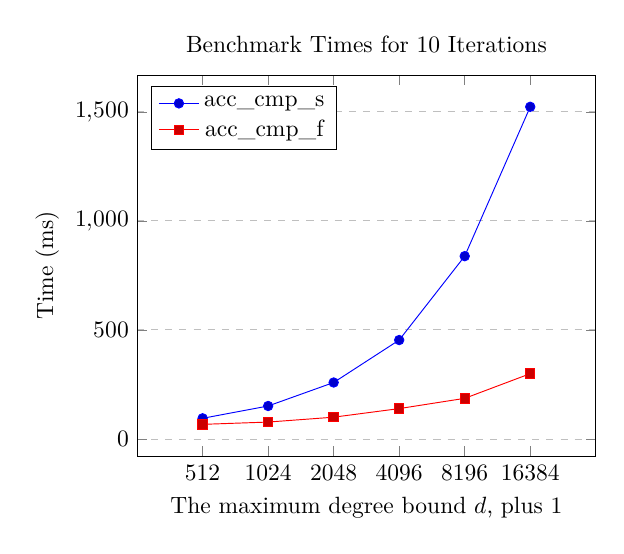
\begin{tikzpicture}[scale=0.85]
    \begin{axis}[
      title={Benchmark Times for 10 Iterations},
      xlabel={The maximum degree bound $d$, plus 1},
      ylabel={Time (ms)},
      xtick=data,
      legend pos=north west,
      ymajorgrids=true,
      grid style=dashed,
      symbolic x coords={512, 1024, 2048, 4096, 8196, 16384},
      enlarge x limits=0.2
    ]
    \addplot coordinates {(512, 94.834) (1024, 151.25) (2048, 258.92) (4096, 453.55) (8196, 838.05) (16384, 1522.7)};
    \addplot coordinates {(512, 67.098) (1024, 77.597) (2048, 99.973) (4096, 139.35) (8196, 186.34) (16384, 299.49)};
    \legend{acc\_cmp\_s, acc\_cmp\_f}
    \end{axis}
    \end{tikzpicture}
  \end{subfigure}
  \begin{subfigure}[b]{0.45\textwidth}
    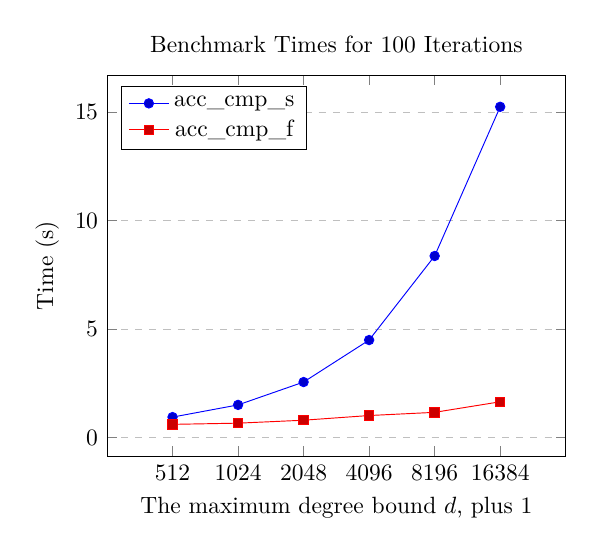
\begin{tikzpicture}[scale=0.85]
      \begin{axis}[
        title={Benchmark Times for 100 Iterations},
        xlabel={The maximum degree bound $d$, plus 1},
        ylabel={Time (s)},
        xtick=data,
        legend pos=north west,
        ymajorgrids=true,
        grid style=dashed,
        symbolic x coords={512, 1024, 2048, 4096, 8196, 16384},
        enlarge x limits=0.2
      ]
      \addplot coordinates {(512, 0.941) (1024, 1.504) (2048, 2.558) (4096, 4.495) (8196, 8.372) (16384, 15.253)};
      \addplot coordinates {(512, 0.607) (1024, 0.662) (2048, 0.798) (4096, 1.014) (8196, 1.161) (16384, 1.648)};
      \legend{acc\_cmp\_s, acc\_cmp\_f}
      \end{axis}
    \end{tikzpicture}
  \end{subfigure}

  \vspace*{10px}

  \begin{subfigure}[b]{0.45\textwidth}
    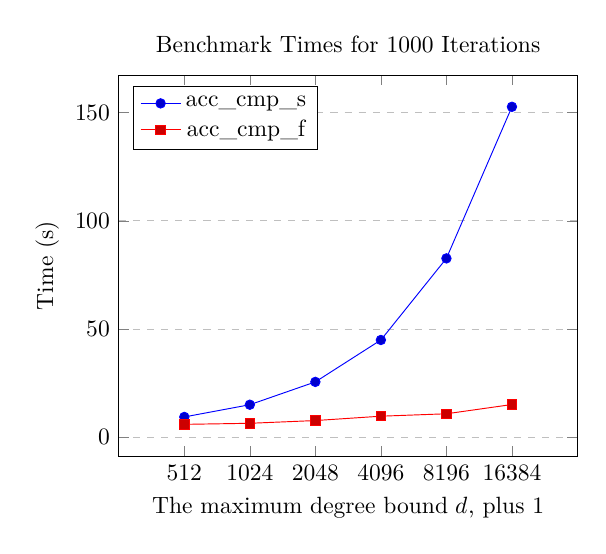
\begin{tikzpicture}[scale=0.85]
    \begin{axis}[
      title={Benchmark Times for 1000 Iterations},
      xlabel={The maximum degree bound $d$, plus 1},
      ylabel={Time (s)},
      xtick=data,
      legend pos=north west,
      ymajorgrids=true,
      grid style=dashed,
      symbolic x coords={512, 1024, 2048, 4096, 8196, 16384},
      enlarge x limits=0.2
    ]
    \addplot coordinates {(512, 9.4381) (1024, 15.087) (2048, 25.621) (4096, 44.970) (8196, 82.643) (16384, 152.63)};
    \addplot coordinates {(512, 6.0183) (1024, 6.5114) (2048, 7.7752) (4096, 9.7851) (8196, 10.899) (16384, 15.176)};
    \legend{acc\_cmp\_s, acc\_cmp\_f}
    \end{axis}
    \end{tikzpicture}
  \end{subfigure}
\end{figure}

Unsurprisingly, increasing the number of iterations only changes the
performance difference up to a certain point, as the difference between
running the decider gets amortized away as the number of iterations
approaches infinity. Also, as was hoped for in the beginning of the
project, the performance of the two approaches show the expected
theoretical runtimes. The \(\vec{G}\) is represented as a constant in
the code, as such, increasing the length of \(\vec{G}\) significantly
above 16,384 leads to slow compilation and failing LSP's. If not for
this fact, testing higher degrees would have been preferred. The
solution is to generate a much larger \(\vec{G}\) at compile-time,
including it in the binary, and reading it as efficiently as possible
during runtime, but this was not done due to time constraints.

\newpage

\section{Appendix}\label{appendix}

\subsection{Notation}\label{notation}

\begin{longtable}[]{@{}
  >{\raggedright\arraybackslash}p{(\columnwidth - 2\tabcolsep) * \real{0.4309}}
  >{\raggedright\arraybackslash}p{(\columnwidth - 2\tabcolsep) * \real{0.5691}}@{}}
\toprule\noalign{}
\endhead
\bottomrule\noalign{}
\endlastfoot
\([n]\) & Denotes the integers \(\{ 1, ..., n \}\) \\
\(a \in \Fb_q\) & A field element in a prime field of order \(q\) \\
\(\vec{a} \in S^n_q\) & A vector of length \(n\) consisting of elements
from set \(S\) \\
\(G \in \Eb(\Fb_q)\) & An elliptic Curve point, defined over field
\(\Fb_q\) \\
\((a_1, \dots, a_n) = [x_i]^n = [x_i]_{i=1}^n = \vec{a} \in S^n_q\) & A
vector of length \(n\) \\
\(v^{(0)}\) & The singular element of a fully compressed vector
\(\vec{v_{\lg(n)}}\) from \(\PCDLOpen\). \\
\(a \in_R S\) & \(a\) is a uniformly randomly sampled element of
\(S\) \\
\((S_1, \dots, S_n)\) & In the context of sets, the same as
\(S_1 \times \dots \times S_n\) \\
\(\dotp{\vec{a}}{\vec{G}}\) where
\(\vec{a} \in \Fb^n_q, \vec{G} \in \Eb^n(\Fb_q)\) & The dot product of
\(\vec{a}\) and \(\vec{G}\) (\(\sum^n_{i=0} a_i G_i\)). \\
\(\dotp{\vec{a}}{\vec{b}}\) where
\(\vec{a} \in \Fb^n_q, \vec{b} \in \Fb^n_q\) & The dot product of
vectors \(\vec{a}\) and \(\vec{b}\). \\
\(l(\vec{a})\) & Gets the left half of \(\vec{a}\). \\
\(r(\vec{a})\) & Gets the right half of \(\vec{a}\). \\
\(\vec{a} \cat \vec{b}\) where
\(\vec{a} \in \Fb^n_q, \vec{b} \in \Fb^m_q\) & Concatenate vectors to
create \(\vec{c} \in \Fb^{n+m}_q\). \\
\(a \cat b\) where \(a \in \Fb_q\) & Create vector
\(\vec{c} = (a, b)\). \\
I.K \(w\) & ``I Know'', Used in the context of proof claims, meaning I
have knowledge of the witness \(w\) \\
\(\Option(T)\) & \(\{ T, \bot \}\) \\
\(\Result(T, E)\) & \(\{ T, E \}\) \\
\(\EvalProof\) &
\((\Eb^{lg(n)}(\Fb_q), \Eb^{lg(n)}(\Fb_q), \Eb(\Fb_q), \Fb_q\mathblue{, \Eb(\Fb_q), \Fb_q})\) \\
\(\AccHiding\) & \((\Eb(\Fb_q), \Nb, \Fb_q, \Fb^d_q)\) \\
\(\Acc\) &
\(((\Eb(\Fb_q), \Nb, \Fb_q, \Fb_q, \EvalProof), \AccHiding)\) \\
\end{longtable}

Note that the following are isomorphic
\(\{ \top, \bot \} \iso \Option(\top) \iso
\Result(\top, \bot)\), but they have different connotations. Generally
for this report, \(\Option(T)\) models optional arguments, where
\(\bot\) indicates an empty argument and \(\Result(T, \bot)\) models the
result of a computation that may fail, particularly used for rejecting
verifiers.

\subsection{Raw Benchmarking Data}\label{raw-benchmarking-data}

The raw benchmarking data provided by Criterion.

\begin{Shaded}
\begin{Highlighting}[]
\NormalTok{  acc\_cmp\_s\_512\_10        time:   [94.245 ms 94.834 ms 95.584 ms]}
\NormalTok{  acc\_cmp\_s\_1024\_10       time:   [150.47 ms 151.25 ms 152.39 ms]}
\NormalTok{  acc\_cmp\_s\_2048\_10       time:   [257.25 ms 258.92 ms 261.14 ms]}
\NormalTok{  acc\_cmp\_s\_4096\_10       time:   [451.60 ms 453.55 ms 456.18 ms]}
\NormalTok{  acc\_cmp\_s\_8196\_10       time:   [833.82 ms 838.05 ms 843.10 ms]}
\NormalTok{  acc\_cmp\_s\_16384\_10      time:   [1.5172 s 1.5227 s 1.5292 s]}
\NormalTok{  acc\_cmp\_f\_512\_10        time:   [66.989 ms 67.098 ms 67.220 ms]}
\NormalTok{  acc\_cmp\_f\_1024\_10       time:   [77.033 ms 77.597 ms 78.330 ms]}
\NormalTok{  acc\_cmp\_f\_2048\_10       time:   [99.415 ms 99.973 ms 100.68 ms]}
\NormalTok{  acc\_cmp\_f\_4096\_10       time:   [138.50 ms 139.35 ms 140.44 ms]}
\NormalTok{  acc\_cmp\_f\_8196\_10       time:   [185.41 ms 186.34 ms 187.59 ms]}
\NormalTok{  acc\_cmp\_f\_16384\_10      time:   [297.72 ms 299.49 ms 301.88 ms]}
\NormalTok{  acc\_cmp\_s\_512\_100       time:   [937.12 ms 940.91 ms 945.67 ms]}
\NormalTok{  acc\_cmp\_s\_1024\_100      time:   [1.4986 s 1.5042 s 1.5107 s]}
\NormalTok{  acc\_cmp\_s\_2048\_100      time:   [2.5490 s 2.5579 s 2.5681 s]}
\NormalTok{  acc\_cmp\_s\_4096\_100      time:   [4.4822 s 4.4945 s 4.5077 s]}
\NormalTok{  acc\_cmp\_s\_8196\_100      time:   [8.2672 s 8.3723 s 8.5111 s]}
\NormalTok{  acc\_cmp\_s\_16384\_100     time:   [15.240 s 15.253 s 15.271 s]}
\NormalTok{  acc\_cmp\_f\_512\_100       time:   [604.98 ms 607.28 ms 610.61 ms]}
\NormalTok{  acc\_cmp\_f\_1024\_100      time:   [658.74 ms 662.03 ms 666.03 ms]}
\NormalTok{  acc\_cmp\_f\_2048\_100      time:   [795.23 ms 798.48 ms 802.54 ms]}
\NormalTok{  acc\_cmp\_f\_4096\_100      time:   [1.0099 s 1.0142 s 1.0194 s]}
\NormalTok{  acc\_cmp\_f\_8196\_100      time:   [1.1559 s 1.1611 s 1.1671 s]}
\NormalTok{  acc\_cmp\_f\_16384\_100     time:   [1.6414 s 1.6484 s 1.6564 s]}
\NormalTok{  acc\_cmp\_s\_512\_1000      time:   [9.4209 s 9.4381 s 9.4555 s]}
\NormalTok{  acc\_cmp\_s\_1024\_1000     time:   [15.059 s 15.087 s 15.135 s]}
\NormalTok{  acc\_cmp\_s\_2048\_1000     time:   [25.604 s 25.621 s 25.638 s]}
\NormalTok{  acc\_cmp\_s\_4096\_1000     time:   [44.951 s 44.970 s 44.990 s]}
\NormalTok{  acc\_cmp\_s\_8196\_1000     time:   [82.605 s 82.643 s 82.697 s]}
\NormalTok{  acc\_cmp\_s\_16384\_1000    time:   [152.43 s 152.63 s 152.93 s]}
\NormalTok{  acc\_cmp\_f\_512\_1000      time:   [6.0046 s 6.0183 s 6.0325 s]}
\NormalTok{  acc\_cmp\_f\_1024\_1000     time:   [6.4971 s 6.5114 s 6.5262 s]}
\NormalTok{  acc\_cmp\_f\_2048\_1000     time:   [7.7599 s 7.7752 s 7.7906 s]}
\NormalTok{  acc\_cmp\_f\_4096\_1000     time:   [9.7686 s 9.7851 s 9.8022 s]}
\NormalTok{  acc\_cmp\_f\_8196\_1000     time:   [10.887 s 10.899 s 10.910 s]}
\NormalTok{  acc\_cmp\_f\_16384\_1000    time:   [15.166 s 15.176 s 15.186 s]}
\end{Highlighting}
\end{Shaded}

\subsection{\texorpdfstring{\(\mathrm{CM}\): Pedersen
Commitment}{\textbackslash mathrm\{CM\}: Pedersen Commitment}}\label{mathrmcm-pedersen-commitment}

As a reference, the Pedersen Commitment algorithm used is included:

\begin{algorithm}[H]
\caption{$\CMCommit$}
\textbf{Inputs} \\
  \Desc{$\vec{m}: \Fb^n$}{The vectors we wish to commit to.} \\
  \Desc{$\vec{G}: \Eb(\Fb)^n$}{The generators we use to create the commitment. From $\pp$.} \\
  \Desc{$\mathblue{\o}: \Option(\Fb_q)$}{Optional hiding factor for the commitment.} \\
\textbf{Output} \\
  \Desc{$C: \Eb(\Fb_q)$}{The Pedersen commitment.}
\begin{algorithmic}[1]
  \State Output $C := \ip{\vec{m}}{\vec{G}} \mathblue{+ \o S}$.
\end{algorithmic}
\end{algorithm}

And the corresponding setup algorithm:

\begin{algorithm}[H]
\caption{$\CMSetup^{\rho_0}$}
\textbf{Inputs} \\
  \Desc{$\l: \Nb$}{The security parameter, in unary form.} \\
  \Desc{$L: \Nb$}{The message format, representing the maximum size vector that can be committed to.} \\
\textbf{Output} \\
  \Desc{$\pp_\CM$}{The public parameters to be used in $\CMCommit$}
\begin{algorithmic}[1]
  \State $(\Gb, q, G) \from \text{SampleGroup}^{\rho_0}(1^\l)$
  \State Choose independently uniformly-sampled generators in $\Gb$, $\vec{G} \in_R \Gb^L, S \in_R \Gb$ using $\rho_0$.
  \State Output $\pp_\CM = ((\Gb, q, G), \vec{G}, S)$
\end{algorithmic}
\end{algorithm}

\newpage

\section*{References}\label{references}
\addcontentsline{toc}{section}{References}

\phantomsection\label{refs}
\begin{CSLReferences}{1}{1}
\bibitem[\citeproctext]{ref-attema}
\textsc{Attema, T., Fehr, S., and Klooß, M.} 2023. Fiat--shamir
transformation of multi-round interactive proofs (extended version).
\url{https://doi.org/10.1007/s00145-023-09478-y}.

\bibitem[\citeproctext]{ref-forking-lemma}
\textsc{Bellare, M., Dai, W., and Li, L.} 2019. The local forking lemma
and its application to deterministic encryption.
\url{https://eprint.iacr.org/2019/1017}.

\bibitem[\citeproctext]{ref-halo}
\textsc{Bowe, S., Grigg, J., and Hopwood, D.} 2019. Recursive proof
composition without a trusted setup.
\url{https://eprint.iacr.org/2019/1021}.

\bibitem[\citeproctext]{ref-bulletproofs}
\textsc{Bünz, B., Bootle, J., Boneh, D., Poelstra, A., Wuille, P., and
Maxwell, G.} 2017. Bulletproofs: Short proofs for confidential
transactions and more. \url{https://eprint.iacr.org/2017/1066}.

\bibitem[\citeproctext]{ref-pcd}
\textsc{Bünz, B., Chiesa, A., Mishra, P., and Spooner, N.} 2020.
Proof-carrying data from accumulation schemes.
\url{https://eprint.iacr.org/2020/499}.

\bibitem[\citeproctext]{ref-ipa}
\textsc{Bünz, B., Maller, M., Mishra, P., Tyagi, N., and Vesely, P.}
2019. Proofs for inner pairing products and applications.
\url{https://eprint.iacr.org/2019/1177}.

\bibitem[\citeproctext]{ref-marlin}
\textsc{Chiesa, A., Hu, Y., Maller, M., Mishra, P., Vesely, P., and
Ward, N.} 2019. Marlin: Preprocessing {zkSNARKs} with universal and
updatable {SRS}. \url{https://eprint.iacr.org/2019/1047}.

\bibitem[\citeproctext]{ref-plonk}
\textsc{Gabizon, A., Williamson, Z.J., and Ciobotaru, O.} 2019. {PLONK}:
Permutations over lagrange-bases for oecumenical noninteractive
arguments of knowledge. \url{https://eprint.iacr.org/2019/953}.

\bibitem[\citeproctext]{ref-from0k2bp}
\textsc{Gibson, A.} 2022. From zero (knowledge) to bulletproofs.
\url{https://github.com/AdamISZ/from0k2bp/blob/8f423712b685246a6be264b7c8081c408e957e67/from0k2bp.pdf}
(Accessed: 2025-01-29).

\bibitem[\citeproctext]{ref-repo}
\textsc{Jakobsen, R.K.} 2025. The project repository.
\url{https://github.com/rasmus-kirk/halo-accumulation} (Accessed:
2025-01-29).

\bibitem[\citeproctext]{ref-hacspec-bulletproofs}
\textsc{Jakobsen, R.K. and Larsen, A.W.} 2022. High assurance
cryptography: Implementing bulletproofs in hacspec.
\url{https://rasmuskirk.com/documents/high-assurance-cryptography-implementing-bulletproofs-in-hacspec.pdf}
(Accessed: 2025-01-29).

\bibitem[\citeproctext]{ref-kzg}
\textsc{Kate, A., Zaverucha, G.M., and Goldberg, I.} 2010.
\href{https://doi.org/10.1007/978-3-642-17373-8_11}{Constant-size
commitments to polynomials and their applications}. \emph{Advances in
cryptology - ASIACRYPT 2010 - 16th international conference on the
theory and application of cryptology and information security},
Springer, 177--194.

\bibitem[\citeproctext]{ref-sonic}
\textsc{Maller, M., Bowe, S., Kohlweiss, M., and Meiklejohn, S.} 2019.
Sonic: Zero-knowledge {SNARKs} from linear-size universal and updateable
structured reference strings. \url{https://eprint.iacr.org/2019/099}.

\bibitem[\citeproctext]{ref-mina}
\textsc{The mina blockchain}. 2025. \url{https://minaprotocol.com/}
(Accessed: 2025-01-29).

\bibitem[\citeproctext]{ref-dalek-docs}
\textsc{Valence, H. de, Yun, C., and Oleg Andreev, and}. 2023. Inner
product proof.
\url{https://doc-internal.dalek.rs/develop/bulletproofs/notes/inner_product_proof/}
(Accessed: 2025-01-29).

\bibitem[\citeproctext]{ref-valiant}
\textsc{Valiant, P.} 2008. Incrementally verifiable computation or
proofs of knowledge imply time/space efficiency. \emph{Theory of
cryptography}, Springer Berlin Heidelberg, 1--18.

\end{CSLReferences}

\end{document}
